%%%%%%%%%%%%%%%%%%%%%%%%%%%%%%%%%%%%%%
% The Legrand Orange Book
% LaTeX Template
% Version 2.1.1 (14/2/16)
%
% This template has been downloaded from:
% http://www.LaTeXTemplates.com
%
% Original author:
% Mathias Legrand (legrand.mathias@gmail.com) with modifications by:
% Vel (vel@latextemplates.com)
%
% License:
% CC BY-NC-SA 3.0 (http://creativecommons.org/licenses/by-nc-sa/3.0/)
%
% Compiling this template:
% This template uses biber for its bibliography and makeindex for its index.
% When you first open the template, compile it from the command line with the
% commands below to make sure your LaTeX distribution is configured correctly:
%
% 1) pdflatex main
% 2) makeindex main.idx -s StyleInd.ist
% 3) biber main
% 4) pdflatex main x 2
%
% After this, when you wish to update the bibliography/index use the appropriate
% command above and make sure to compile with pdflatex several times
% afterwards to propagate your changes to the document.
%
% This template also uses a number of packages which may need to be
% updated to the newest versions for the template to compile. It is strongly
% recommended you update your LaTeX distribution if you have any
% compilation errors.
%
% Important note:
% Chapter heading images should have a 2:1 width:height ratio,
% e.g. 920px width and 460px height.
%
%%%%%%%%%%%%%%%%%%%%%%%%%%%%%%%%%%%%%%%%%

%----------------------------------------------------------------------------------------
%	PACKAGES AND OTHER DOCUMENT CONFIGURATIONS
%----------------------------------------------------------------------------------------

%\documentclass[10pt,fleqn]{book} % Default font size and left-justified equations
\documentclass[11pt]{book} % Default font size and left-justified equations

\usepackage[utf8]{inputenc}
\usepackage{graphicx}
\usepackage{epstopdf}
\usepackage{csquotes}
\usepackage{wrapfig}
\usepackage{rotating}
\usepackage{caption}
%\captionsetup{font={small, it}}
\captionsetup{font={small}}
\captionsetup[figure]{font={small}, labelfont={bf}, name={Fig.}}
\captionsetup[table]{font={small}, labelfont={bf}, name={Table}}

\usepackage{imakeidx}
\makeindex
%% \usepackage{draftwatermark}
%% \SetWatermarkText{SR-CU-2020}
%% \SetWatermarkScale{0.9}
%% \SetWatermarkAngle{65}
%% \SetWatermarkHorCenter{0.3\paperwidth}
%% \SetWatermarkVerCenter{0.5\paperwidth}

%\usepackage[paperwidth=6in, paperheight=9in, margin=0.7in]{geometry}
%----------------------------------------------------------------------------------------
%%%%%%%%%%%%%%%%%%%%%%%%%%%%%%%%%%%%%%%%%
% The Legrand Orange Book
% Structural Definitions File
% Version 2.0 (9/2/15)
%
% Original author:
% Mathias Legrand (legrand.mathias@gmail.com) with modifications by:
% Vel (vel@latextemplates.com)
%
% This file has been downloaded from:
% http://www.LaTeXTemplates.com
%
% License:
% CC BY-NC-SA 3.0 (http://creativecommons.org/licenses/by-nc-sa/3.0/)
%
%%%%%%%%%%%%%%%%%%%%%%%%%%%%%%%%%%%%%%%%%

%----------------------------------------------------------------------------------------
%	VARIOUS REQUIRED PACKAGES AND CONFIGURATIONS
%----------------------------------------------------------------------------------------

%\usepackage[top=3cm,bottom=3cm,left=3cm,right=3cm,headsep=10pt,a4paper]{geometry} % Page margins
\usepackage[paperwidth=6in, paperheight=9in, margin=0.8in]{geometry}

\usepackage{graphicx} % Required for including pictures
\graphicspath{{Pictures/}} % Specifies the directory where pictures are stored

%\usepackage{lipsum} % Inserts dummy text

\usepackage{tikz} % Required for drawing custom shapes

\usepackage[english]{babel} % English language/hyphenation

\usepackage{enumitem} % Customize lists
\setlist{nolistsep} % Reduce spacing between bullet points and numbered lists

\usepackage{booktabs} % Required for nicer horizontal rules in tables

\usepackage{xcolor} % Required for specifying colors by name
\definecolor{ocre}{RGB}{243,102,25}
\definecolor{darkocre}{RGB}{250,150,70}

%----------------------------------------------------------------------------------------
%	FONTS
%----------------------------------------------------------------------------------------

\usepackage{avant} % Use the Avantgarde font for headings
%\usepackage{times} % Use the Times font for headings
%\usepackage{mathptmx} % Use the Adobe Times Roman as the default text
                      % font together with math symbols from the
                      % Sym­bol, Chancery and Com­puter Modern fonts
%\usepackage{mathpazo}

\usepackage{lmodern}        % Latin Modern family of fonts -- NOT BAD AT ALL
\usepackage{libertine}  % ok too.
%\usepackage{charter}
% font faces
% lmodern -- latin Modern Roman
% tgtermes -- TeX Gyre Termes
% tgpagella -- TeX Gyre Pagella
% tgbonum -- TeX Gyre Bonum
% tgschola -- Tex Gyr Schola
% mathptmx -- Time
% utopia/fourier -- Utopia/Fourier
% palatino -- Palatino
% bookman -- Bookman
% charter -- Charter

\usepackage{microtype} % Slightly tweak font spacing for aesthetics
\usepackage[utf8]{inputenc} % Required for including letters with accents
\usepackage[T1]{fontenc} % Use 8-bit encoding that has 256 glyphs

% Fancy big letter at the beginning of a chapter
\usepackage{lettrine}
% compact underline
\usepackage[normalem]{ulem}

%----------------------------------------------------------------------------------------
%	BIBLIOGRAPHY AND INDEX
%----------------------------------------------------------------------------------------

\usepackage[style=alphabetic,citestyle=numeric,sorting=nyt,sortcites=true,autopunct=true,babel=hyphen,hyperref=true,abbreviate=false,backref=true,backend=biber]{biblatex}
\addbibresource{bibliography.bib} % BibTeX bibliography file
\defbibheading{bibempty}{}

\usepackage{calc} % For simpler calculation - used for spacing the index letter headings correctly
\usepackage{makeidx} % Required to make an index
\makeindex % Tells LaTeX to create the files required for indexing

% more spacing between lines
\usepackage{setspace}
\setstretch{1.0}

% put formulas in a box
\usepackage{amsmath,amsfonts,amssymb,amsthm} % For math equations, theorems, symbols, etc
\usepackage[most]{tcolorbox}
%\usepackage{MnSymbol}


%----------------------------------------------------------------------------------------
%	MAIN TABLE OF CONTENTS
%----------------------------------------------------------------------------------------

\usepackage{titletoc} % Required for manipulating the table of contents

\contentsmargin{1cm} % Removes the default margin

% Part text styling
\titlecontents{part}[0cm]
%{\addvspace{20pt}\centering\large\bfseries}
{\addvspace{20pt}\centering\bfseries}
{}
{}
{}

% Chapter text styling
\titlecontents{chapter}[1.25cm] % Indentation
{\addvspace{12pt}\large\sffamily\bfseries} % Spacing and font options for chapters
{\color{ocre!60}\contentslabel[\Large\thecontentslabel]{1.25cm}\color{ocre}} % Chapter number
{\color{ocre}}
{\color{ocre!60}\normalsize\;\titlerule*[.5pc]{.}\;\thecontentspage} % Page number

% Section text styling
\titlecontents{section}[1.25cm] % Indentation
{\addvspace{3pt}\sffamily\bfseries} % Spacing and font options for sections
{\contentslabel[\thecontentslabel]{1.25cm}} % Section number
{}
{\hfill\color{black}\thecontentspage} % Page number
[]

% Subsection text styling
\titlecontents{subsection}[1.25cm] % Indentation
{\addvspace{3pt}\sffamily\small} % Spacing and font options for subsections
{\contentslabel[\thecontentslabel]{1.25cm}} % Subsection number
{}
{\ \titlerule*[.5pc]{.}\;\thecontentspage} % Page number
[]

% List of figures
\titlecontents{figure}[0em]
{\addvspace{-5pt}\sffamily}
{\thecontentslabel\hspace*{1em}}
{}
{\ \titlerule*[.5pc]{.}\;\thecontentspage}
[]

% List of tables
\titlecontents{table}[0em]
{\addvspace{-5pt}\sffamily}
{\thecontentslabel\hspace*{1em}}
{}
{\ \titlerule*[.5pc]{.}\;\thecontentspage}
[]

%----------------------------------------------------------------------------------------
%	MINI TABLE OF CONTENTS IN PART HEADS
%----------------------------------------------------------------------------------------

% Chapter text styling
\titlecontents{lchapter}[0em] % Indenting
{\addvspace{15pt}\large\sffamily\bfseries} % Spacing and font options for chapters
{\color{black}\contentslabel[\Large\thecontentslabel]{1.25cm}\color{black}} % Chapter number
{}
{\color{black}\normalsize\sffamily\bfseries\;\titlerule*[.5pc]{.}\;\thecontentspage} % Page number

% Section text styling
\titlecontents{lsection}[0em] % Indenting
{\sffamily\small} % Spacing and font options for sections
{\contentslabel[\thecontentslabel]{1.25cm}} % Section number
{}
{}

% Subsection text styling
\titlecontents{lsubsection}[.5em] % Indentation
{\normalfont\footnotesize\sffamily} % Font settings
{\contentslabel[\thecontentslabel]{1.25cm}} % Section number
{}
{}

%----------------------------------------------------------------------------------------
%	PAGE HEADERS
%----------------------------------------------------------------------------------------

\usepackage{fancyhdr} % Required for header and footer configuration

\pagestyle{fancy}
\renewcommand{\chaptermark}[1]{\markboth{\sffamily\normalsize\bfseries\chaptername\ \thechapter.\ #1}{}} % Chapter text font settings
\renewcommand{\sectionmark}[1]{\markright{\sffamily\normalsize\thesection\hspace{5pt}#1}{}} % Section text font settings
\fancyhf{} \fancyhead[LE,RO]{\sffamily\normalsize\thepage} % Font setting for the page number in the header
\fancyhead[LO]{\rightmark} % Print the nearest section name on the left side of odd pages
\fancyhead[RE]{\leftmark} % Print the current chapter name on the right side of even pages
\renewcommand{\headrulewidth}{0.5pt} % Width of the rule under the header
\addtolength{\headheight}{2.5pt} % Increase the spacing around the header slightly
\renewcommand{\footrulewidth}{0pt} % Removes the rule in the footer
\fancypagestyle{plain}{\fancyhead{}\renewcommand{\headrulewidth}{0pt}} % Style for when a plain pagestyle is specified

% Removes the header from odd empty pages at the end of chapters
\makeatletter
\renewcommand{\cleardoublepage}{
\clearpage\ifodd\c@page\else
\hbox{}
\vspace*{\fill}
\thispagestyle{empty}
\newpage
\fi}

%----------------------------------------------------------------------------------------
%	THEOREM STYLES
%----------------------------------------------------------------------------------------

\newcommand{\intoo}[2]{\mathopen{]}#1\,;#2\mathclose{[}}
\newcommand{\ud}{\mathop{\mathrm{{}d}}\mathopen{}}
\newcommand{\intff}[2]{\mathopen{[}#1\,;#2\mathclose{]}}
\newtheorem{notation}{Notation}[chapter]

% Boxed/framed environments
\newtheoremstyle{ocrenumbox}% % Theorem style name
{0pt}% Space above
{0pt}% Space below
{\normalfont}% % Body font
{}% Indent amount
{\small\bf\sffamily\color{ocre}}% % Theorem head font
{\;}% Punctuation after theorem head
{0.25em}% Space after theorem head
{\small\sffamily\color{ocre}\thmname{#1}\nobreakspace\thmnumber{\@ifnotempty{#1}{}\@upn{#2}}% Theorem text (e.g. Theorem 2.1)
\thmnote{\nobreakspace\the\thm@notefont\sffamily\bfseries\color{black}---\nobreakspace#3.}} % Optional theorem note
\renewcommand{\qedsymbol}{$\blacksquare$}% Optional qed square

\newtheoremstyle{blacknumex}% Theorem style name
{5pt}% Space above
{5pt}% Space below
{\normalfont}% Body font
{} % Indent amount
{\small\bf\sffamily}% Theorem head font
{\;}% Punctuation after theorem head
{0.25em}% Space after theorem head
{\small\sffamily{\tiny\ensuremath{\blacksquare}}\nobreakspace\thmname{#1}\nobreakspace\thmnumber{\@ifnotempty{#1}{}\@upn{#2}}% Theorem text (e.g. Theorem 2.1)
\thmnote{\nobreakspace\the\thm@notefont\sffamily\bfseries---\nobreakspace#3.}}% Optional theorem note

\newtheoremstyle{blacknumbox} % Theorem style name
{0pt}% Space above
{0pt}% Space below
{\normalfont}% Body font
{}% Indent amount
{\small\bf\sffamily}% Theorem head font
{\;}% Punctuation after theorem head
{0.25em}% Space after theorem head
{\small\sffamily\thmname{#1}\nobreakspace\thmnumber{\@ifnotempty{#1}{}\@upn{#2}}% Theorem text (e.g. Theorem 2.1)
\thmnote{\nobreakspace\the\thm@notefont\sffamily\bfseries---\nobreakspace#3.}}% Optional theorem note

% Non-boxed/non-framed environments
\newtheoremstyle{ocrenum}% % Theorem style name
{5pt}% Space above
{5pt}% Space below
{\normalfont}% % Body font
{}% Indent amount
{\small\bf\sffamily\color{ocre}}% % Theorem head font
{\;}% Punctuation after theorem head
{0.25em}% Space after theorem head
{\small\sffamily\color{ocre}\thmname{#1}\nobreakspace\thmnumber{\@ifnotempty{#1}{}\@upn{#2}}% Theorem text (e.g. Theorem 2.1)
\thmnote{\nobreakspace\the\thm@notefont\sffamily\bfseries\color{black}---\nobreakspace#3.}} % Optional theorem note
\renewcommand{\qedsymbol}{$\blacksquare$}% Optional qed square
\makeatother

% Non-boxed/non-framed environments
\newtheoremstyle{bionum}% % Theorem style name
{5pt}% Space above
{5pt}% Space below
{\normalfont}% % Body font
{}% Indent amount
{\small\bf\sffamily\color{blue}}% % Theorem head font
{\;}% Punctuation after theorem head
{0.25em}% Space after theorem head
\makeatother

% Defines the theorem text style for each type of theorem to one of the three styles above
\newcounter{dummy}
\numberwithin{dummy}{section}
\theoremstyle{ocrenumbox}
\newtheorem{theoremeT}[dummy]{Theorem}
\newtheorem{problem}{Problem}[chapter]
\newtheorem{exerciseT}{Exercise}[chapter]
\theoremstyle{blacknumex}
\newtheorem{exampleT}{Example}[chapter]
\theoremstyle{blacknumbox}
\newtheorem{vocabulary}{Vocabulary}[chapter]
\newtheorem{definitionT}{Definition}[chapter]
\newtheorem{corollaryT}[dummy]{Corollary}
\theoremstyle{ocrenum}
\newtheorem{proposition}[dummy]{Proposition}
\theoremstyle{bionum}
\newtheorem{bioT}{Bio}[chapter]
%----------------------------------------------------------------------------------------
%	DEFINITION OF COLORED BOXES
%----------------------------------------------------------------------------------------

%% \RequirePackage[framemethod=default]{mdframed} % Required for creating
%%                                 % the theorem, definition, exercise
%%                                 % and corollary boxes
\RequirePackage[framemethod=TikZ]{mdframed} % Required for creating
                                % the theorem, definition, exercise
                                % and corollary boxes

% Biographt box
\newmdenv[skipabove=7pt,
skipbelow=7pt,
rightline=false,
leftline=true,
topline=false,
bottomline=false,
backgroundcolor=blue!5,
linecolor=blue,
innerleftmargin=5pt,
innerrightmargin=5pt,
innertopmargin=5pt,
innerbottommargin=5pt,
leftmargin=0cm,
rightmargin=0cm,
linewidth=2pt]{bBox}

\newmdenv[skipabove=7pt,
skipbelow=7pt,
rightline=false,
leftline=true,
topline=false,
bottomline=false,
backgroundcolor=green!5,
linecolor=green,
innerleftmargin=5pt,
innerrightmargin=5pt,
innertopmargin=5pt,
innerbottommargin=5pt,
leftmargin=0cm,
rightmargin=0cm,
linewidth=2pt]{rBox}  % reminder


% Theorem box
\newmdenv[skipabove=7pt,
skipbelow=7pt,
backgroundcolor=black!5,
linecolor=ocre,
innerleftmargin=5pt,
innerrightmargin=5pt,
innertopmargin=5pt,
leftmargin=0cm,
rightmargin=0cm,
roundcorner=2pt,
innerbottommargin=5pt]{tBox}

% Exercise box
\newmdenv[skipabove=7pt,
skipbelow=7pt,
rightline=false,
leftline=true,
topline=false,
bottomline=false,
backgroundcolor=ocre!10,
linecolor=ocre,
innerleftmargin=5pt,
innerrightmargin=5pt,
innertopmargin=5pt,
innerbottommargin=5pt,
leftmargin=0cm,
rightmargin=0cm,
linewidth=4pt]{eBox}

% Definition box
\newmdenv[skipabove=7pt,
skipbelow=7pt,
%rightline=false,
%leftline=true,
%topline=false,
%bottomline=false,
backgroundcolor=green!10,
linecolor=green,
innerleftmargin=5pt,
innerrightmargin=5pt,
innertopmargin=5pt,
innerbottommargin=10pt,
leftmargin=0cm,
rightmargin=0cm,
%linewidth=4pt,
roundcorner=2,
innerbottommargin=0pt]{dBox}

% Corollary box
\newmdenv[skipabove=7pt,
skipbelow=7pt,
rightline=false,
leftline=true,
topline=false,
bottomline=false,
linecolor=gray,
backgroundcolor=black!5,
innerleftmargin=5pt,
innerrightmargin=5pt,
innertopmargin=5pt,
leftmargin=0cm,
rightmargin=0cm,
linewidth=4pt,
innerbottommargin=5pt]{cBox}

% Prerequisite box
\newmdenv[skipabove=7pt,
skipbelow=7pt,
%rightline=false,
%leftline=true,
%topline=false,
%bottomline=false,
backgroundcolor=magenta!8,
linecolor=black!20,
innerleftmargin=5pt,
innerrightmargin=5pt,
innertopmargin=5pt,
innerbottommargin=10pt,
leftmargin=0cm,
rightmargin=0cm,
%linewidth=4pt,
roundcorner=2,
innerbottommargin=0pt]{prBox}


% Example box
\newmdenv[skipabove=7pt,
skipbelow=7pt,
%rightline=false,
%leftline=true,
%topline=false,
%bottomline=false,
backgroundcolor=cyan!8,
linecolor=black!20,
innerleftmargin=5pt,
innerrightmargin=5pt,
innertopmargin=5pt,
innerbottommargin=10pt,
leftmargin=0cm,
rightmargin=0cm,
%linewidth=4pt,
roundcorner=2,
innerbottommargin=0pt]{exBox}


% Creates an environment for each type of theorem and assigns it a theorem text style from the "Theorem Styles" section above and a colored box from above
\newenvironment{theorem}{\begin{tBox}\begin{theoremeT}}{\end{theoremeT}\end{tBox}}
%% \newenvironment{exercise}{\begin{eBox}\begin{exerciseT}\faPencilSquareO\\}{\hfill{\color{ocre}\tiny\ensuremath{\blacksquare}}\end{exerciseT}\end{eBox}}
\newenvironment{exercise}{\begin{eBox}\begin{exerciseT}\faPencilSquareO\\}{\hfill{\color{ocre}\faPencilSquare}\end{exerciseT}\end{eBox}}
\newenvironment{definition}{\begin{dBox}\begin{definitionT}}{\end{definitionT}\end{dBox}}

\newenvironment{example}{\begin{exampleT}}{\hfill{\tiny\ensuremath{\blacksquare}}\end{exampleT}}
\newenvironment{corollary}{\begin{cBox}\begin{corollaryT}}{\end{corollaryT}\end{cBox}}
\newenvironment{bio}{\begin{bBox}\begin{bioT}}{\end{bioT}\end{bBox}}


% my additions
%% \newenvironment{myexercise}
%%     {\begin{eBox}\begin{exerciseT}}\faPencilSquareO
%%         {\hfill{\color{ocre}\tiny\ensuremath{\blacksquare}}
%%         \end{exerciseT}\end{eBox}
%%         }

%----------------------------------------------------------------------------------------
%	REMARK ENVIRONMENT
%----------------------------------------------------------------------------------------

\newenvironment{remark}{\par\vspace{10pt}\small % Vertical white space above the remark and smaller font size
\begin{list}{}{
\leftmargin=35pt % Indentation on the left
\rightmargin=25pt}\item\ignorespaces % Indentation on the right
\makebox[-2.5pt]{\begin{tikzpicture}[overlay]
\node[draw=ocre!60,line width=1pt,circle,fill=ocre!25,font=\sffamily\bfseries,inner sep=2pt,outer sep=0pt] at (-15pt,0pt){\textcolor{ocre}{R}};\end{tikzpicture}} % Orange R in a circle
\advance\baselineskip -1pt}{\end{list}\vskip5pt} % Tighter line spacing and white space after remark

%----------------------------------------------------------------------------------------
%	INFO ENVIRONMENT
%----------------------------------------------------------------------------------------

\newenvironment{info}{\par\vspace{10pt}\small % Vertical white space above the remark and smaller font size
\begin{list}{}{
\leftmargin=35pt % Indentation on the left
\rightmargin=25pt}\item\ignorespaces % Indentation on the right
\makebox[-2.5pt]{\begin{tikzpicture}[overlay]
\node[draw=blue!60,line width=1pt,circle,fill=gray!25,font=\sffamily\bfseries,inner sep=2pt,outer sep=0pt] at (-15pt,0pt){\textcolor{blue}{I}};\end{tikzpicture}} % Orange R in a circle
\advance\baselineskip -1pt}{\end{list}\vskip5pt} % Tighter line spacing and white space after remark

%----------------------------------------------------------------------------------------
%	SECTION NUMBERING IN THE MARGIN
%----------------------------------------------------------------------------------------

\makeatletter
\renewcommand{\@seccntformat}[1]{\llap{\textcolor{black}{\csname the#1\endcsname}\hspace{1em}}}

\renewcommand{\section}{\@startsection{section}{1}{0.5in}
{-4ex \@plus -1ex \@minus -.4ex}
{1ex \@plus.2ex }
{\normalfont\large\bfseries}}
%{\normalfont\large\sffamily\bfseries}}

\renewcommand{\subsection}{\@startsection {subsection}{2}{0.5in}
{-3ex \@plus -0.1ex \@minus -.4ex}
{0.5ex \@plus.2ex }
{\normalfont\bfseries}}

\renewcommand{\subsubsection}{\@startsection {subsubsection}{3}{\z@}
{-2ex \@plus -0.1ex \@minus -.2ex}
{.2ex \@plus.2ex }
{\normalfont\small\bfseries}}

\renewcommand{\paragraph}{\@startsection{paragraph}{4}{0.5in}
{-2ex \@plus-.2ex \@minus .2ex}
{.1ex}
{\normalfont\small\sffamily\bfseries}}

%----------------------------------------------------------------------------------------
%	PART HEADINGS
%----------------------------------------------------------------------------------------

% numbered part in the table of contents
\newcommand{\@mypartnumtocformat}[2]{%
\setlength\fboxsep{0pt}%
\noindent\colorbox{ocre!20}{\strut\parbox[c][.7cm]{\ecart}{\color{ocre!70}\large\sffamily\bfseries\centering#1}}\hskip\esp\colorbox{ocre!40}{\strut\parbox[c][.7cm]{\linewidth-\ecart-\esp}{\large\sffamily\centering#2}}}%
%%%%%%%%%%%%%%%%%%%%%%%%%%%%%%%%%%
% unnumbered part in the table of contents
\newcommand{\@myparttocformat}[1]{%
\setlength\fboxsep{0pt}%
\noindent\colorbox{ocre!40}{\strut\parbox[c][.7cm]{\linewidth}{\large\sffamily\centering#1}}}%
%%%%%%%%%%%%%%%%%%%%%%%%%%%%%%%%%%
\newlength\esp
\setlength\esp{4pt}
\newlength\ecart
\setlength\ecart{1.2cm-\esp}
\newcommand{\thepartimage}{}%
\newcommand{\partimage}[1]{\renewcommand{\thepartimage}{#1}}%
\def\@part[#1]#2{%
\ifnum \c@secnumdepth >-2\relax%
\refstepcounter{part}%
\addcontentsline{toc}{part}{\texorpdfstring{\protect\@mypartnumtocformat{\thepart}{#1}}{\partname~\thepart\ ---\ #1}}
\else%
\addcontentsline{toc}{part}{\texorpdfstring{\protect\@myparttocformat{#1}}{#1}}%
\fi%
\startcontents%
\markboth{}{}%
{\thispagestyle{empty}%
\begin{tikzpicture}[remember picture,overlay]%
\node at (current page.north west){\begin{tikzpicture}[remember picture,overlay]%
\fill[ocre!20](0cm,0cm) rectangle (\paperwidth,-\paperheight);
\node[anchor=north] at (3cm,-3.25cm){\color{ocre!40}\fontsize{110}{50}\sffamily\bfseries\@Roman\c@part};
\node[anchor=south east] at (\paperwidth-1cm,-\paperheight+1cm){\parbox[t][][t]{8.5cm}{
\printcontents{l}{0}{\setcounter{tocdepth}{1}}%
}};
\node[anchor=north east] at (\paperwidth-1.5cm,-3.25cm){\parbox[t][][t]{15cm}{\strut\raggedleft\color{black}\fontsize{30}{30}\sffamily\bfseries#2}};
\end{tikzpicture}};
\end{tikzpicture}}%
\@endpart}
\def\@spart#1{%
\startcontents%
\phantomsection
{\thispagestyle{empty}%
\begin{tikzpicture}[remember picture,overlay]%
\node at (current page.north west){\begin{tikzpicture}[remember picture,overlay]%
\fill[ocre!20](0cm,0cm) rectangle (\paperwidth,-\paperheight);
\node[anchor=north east] at (\paperwidth-1.5cm,-3.25cm){\parbox[t][][t]{15cm}{\strut\raggedleft\color{white}\fontsize{30}{30}\sffamily\bfseries#1}};
\end{tikzpicture}};
\end{tikzpicture}}
\addcontentsline{toc}{part}{\texorpdfstring{%
\setlength\fboxsep{0pt}%
\noindent\protect\colorbox{ocre!40}{\strut\protect\parbox[c][.7cm]{\linewidth}{\Large\sffamily\protect\centering #1\quad\mbox{}}}}{#1}}%
\@endpart}
\def\@endpart{\vfil\newpage
\if@twoside
\if@openright
\null
\thispagestyle{empty}%
\newpage
\fi
\fi
\if@tempswa
\twocolumn
\fi}

%----------------------------------------------------------------------------------------
%	CHAPTER HEADINGS
%----------------------------------------------------------------------------------------

% A switch to conditionally include a picture, implemented by  Christian Hupfer
\newif\ifusechapterimage
\usechapterimagetrue
\newcommand{\thechapterimage}{}%
\newcommand{\chapterimage}[1]{\ifusechapterimage\renewcommand{\thechapterimage}{#1}\fi}%
\def\@makechapterhead#1{%
{\parindent \z@ \raggedright \normalfont
\ifnum \c@secnumdepth >\m@ne
\if@mainmatter
\begin{tikzpicture}[remember picture,overlay]
\node at (current page.north west)
{\begin{tikzpicture}[remember picture,overlay]
\node[anchor=north west,inner sep=0pt] at (0,0) {\ifusechapterimage\includegraphics[width=\paperwidth]{\thechapterimage}\fi};
%\draw[anchor=west] (\Gm@lmargin, -8.5cm) node [line width=2pt,rounded corners=5pt,draw=ocre,fill=white,fill opacity=0.3,inner sep=15pt]{\strut\makebox[22cm]{}};
\draw[anchor=west] (\Gm@lmargin+.3cm,-7.0cm) node {\huge\sffamily\bfseries\color{black}\thechapter. #1\strut};
\end{tikzpicture}};
\end{tikzpicture}
\else
\begin{tikzpicture}[remember picture,overlay]
\node at (current page.north west)
{\begin{tikzpicture}[remember picture,overlay]
\node[anchor=north west,inner sep=0pt] at (0,0) {\ifusechapterimage\includegraphics[width=\paperwidth]{\thechapterimage}\fi};
%\draw[anchor=west] (\Gm@lmargin,-9cm) node [line width=2pt,rounded corners=15pt,draw=ocre,fill=white,fill opacity=0.5,inner sep=15pt]{\strut\makebox[22cm]{}};
\draw[anchor=west] (\Gm@lmargin+.3cm,-9cm) node {\huge\sffamily\bfseries\color{black}#1\strut};
\end{tikzpicture}};
\end{tikzpicture}
\fi\fi\par\vspace*{145\p@}}}

%-------------------------------------------

\def\@makeschapterhead#1{%
\begin{tikzpicture}[remember picture,overlay]
\node at (current page.north west)
{\begin{tikzpicture}[remember picture,overlay]
\node[anchor=north west,inner sep=0pt] at (0,0) {\ifusechapterimage\includegraphics[width=\paperwidth]{\thechapterimage}\fi};
%\draw[anchor=west] (\Gm@lmargin,-9cm) node [line width=2pt,rounded corners=15pt,draw=ocre,fill=white,fill opacity=0.5,inner sep=15pt]{\strut\makebox[22cm]{}};
\draw[anchor=west] (\Gm@lmargin+.3cm,-9cm) node {\huge\sffamily\bfseries\color{black}#1\strut};
\end{tikzpicture}};
\end{tikzpicture}
\par\vspace*{270\p@}}
\makeatother

%----------------------------------------------------------------------------------------
%	HYPERLINKS IN THE DOCUMENTS
%----------------------------------------------------------------------------------------

\usepackage{hyperref}
\hypersetup{hidelinks,backref=true,pagebackref=true,hyperindex=true,colorlinks=false,breaklinks=true,urlcolor= ocre,bookmarks=true,bookmarksopen=false,pdftitle={Title},pdfauthor={Author}}
\usepackage{bookmark}
\bookmarksetup{
open,
numbered,
addtohook={%
\ifnum\bookmarkget{level}=0 % chapter
\bookmarksetup{bold}%
\fi
\ifnum\bookmarkget{level}=-1 % part
\bookmarksetup{color=ocre,bold}%
\fi
}
}

% additional fonts
\usepackage{fontawesome}
\usepackage{MnSymbol}

%\usepackage[table,xcdraw]{xcolor}

%\newcommand{\tus}{\text{\,\textunderscore\,}}

% this one worked superbly!
%\newcommand{\tus}{\text{\,\textcolor{lightgray}{$\bullet$}\,}}
% when printed the color is too light when lightgray
\newcommand{\tus}{\text{\,\textcolor{gray}{$\bullet$}\,}}


\newcommand{\qs}[1]{|{#1}\rangle}  % quantum state
\newcommand{\ket}[1]{|{#1}\rangle}  % quantum state
\newcommand{\bra}[1]{\langle{#1}|}  % quantum state
\newcommand{\braket}[2]{\langle{#1}|{#2\rangle}}  % quantum bracket
\newcommand{\ketbra}[2]{|{#1}\rangle\langle{#2}|}  % quantum bracket


\newcommand{\ms}[1]{\overset{\rightharpoonup}{#1}}
%\newcommand{\op}[1]{\overset{\land}{#1}}
%\newcommand{\op}[1]{\overset{\sqfrown}{#1}}
\newcommand{\op}[1]{\widehat{#1}}  % operator hat

\newcommand{\proj}[1]{\uuline{#1}}  % projector
\newcommand{\projop}[1]{\op{\proj{#1}}}  % projector operator

\newcommand{\vsp}[1]{\overset{\Rightarrow}{#1}}  % vector space
\newcommand{\vspd}[1]{\overset{\Leftarrow}{#1}}  % dual vector space
\newcommand{\vecp}[1]{\vec{#1}\,'}  % vector primed
\newcommand{\vecl}[1]{\overset{\leftarrow}{#1}}  % dual --- vector with arrow left
\newcommand{\veclp}[1]{\overset{\leftarrow}{#1}\,'}  % dual --- vector with arrow left
\renewcommand{\vec}[1]{\overset{\rightarrow}{#1}}  % vector
%\newcommand{}[1]{\overset{\land}{#1}}
%\newcommand{\proj}[1]{\overset{\leftrightarrow}{#1}}  % vector space

\newcommand{\bem}[1]{{\bf\emph{#1}}}

\newenvironment{mybio}[1]{\begin{bBox}\begin{bioT}\faBook\,\,\bem{#1}\\}
                         {\vspace{0.1cm}\end{bioT}\end{bBox}}
\newenvironment{myrem}[1]{\begin{rBox}\faExclamationCircle\,\,\bem{#1}\\}
                         {\end{rBox}}
%\newenvironment{mydef}[1]{\begin{dBox}\begin{definitionT}\faGraduationCap\,\,\bem{#1}\\}{\end{definitionT}\end{dBox}}
\newenvironment{mydef}[1]{\begin{dBox}\begin{definitionT}\faHandORight\,\,\bem{#1}\\}{\vspace{0.2cm}\end{definitionT}\end{dBox}}

\newenvironment{analogy}{\begin{tBox}\faSunO\,\,\bem{Analogy}\\}{\vspace{0.1cm}\end{tBox}}
\newenvironment{myExample}{\begin{exBox}\faCommentO\,\,\bem{Example}\\}{\vspace{0.1cm}\end{exBox}}


\newenvironment{myprereq}[1]{\begin{prBox}\begin{bioT}\faCheckSquareO\,\,\bem{#1}\\}
		{\vspace{0.1cm}\end{bioT}\end{prBox}}

\newcommand{\chhc}{\color{blue!10!black}}

%% COLORED BOXES FOR FORMULAE
\setlength\fboxrule{1pt}
% Syntax: \colorboxed[<color model>]{<color specification>}{<math formula>}
\newcommand*{\colorboxed}{}
\def\colorboxed#1#{%
  \colorboxedAux{#1}%
}
\newcommand*{\colorboxedAux}[3]{%
  % #1: optional argument for color model
  % #2: color specification
  % #3: formula
  \begingroup
    \colorlet{cb@saved}{.}%
    \color#1{#2}%
    \boxed{%
      \color{cb@saved}%
      #3%
    }%
  \endgroup
}

% bold text command
\newcommand{\btc}[1]{\textrm{\bf {#1}}}
 % Insert the commands.tex file which contains the majority of the structure behind the template
\usepackage{mathtools}
\usepackage[outercaption]{sidecap}  % some captions needed at the side \begin{SCfigure}
\begin{document}

% uncomment to build e-book version
%----
%  FRONT COVER
%---------
\begingroup
\thispagestyle{empty}
\begin{tikzpicture}[remember picture,overlay]
\coordinate [below=0cm] (midpoint) at (current page.north);
\node at (current page.north west)
{\begin{tikzpicture}[remember picture,overlay]
\node[anchor=north west,inner sep=0pt] at (0,0) {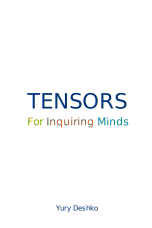
\includegraphics[width=\paperwidth]{pics/bookCoverInner_Var1}}; % Background image
%\draw[anchor=north] (midpoint) node [fill=ocre!30!white,fill opacity=0.6,text opacity=1,inner sep=1cm]{\Huge\centering\bfseries\sffamily\parbox[c][][t]{\paperwidth}{\centering Relativity\\[15pt] % Book title
%{\Large For the Inquiring Mind}\\[20pt] % Subtitle
%{\huge Dr. Yury Deshko}}}; % Author name
\end{tikzpicture}};
\end{tikzpicture}
\vfill
\endgroup
\newpage

%----------------------------------------------------------------------------------------
%	COPYRIGHT PAGE
%----------------------------------------------------------------------------------------

~\vfill
\thispagestyle{empty}
\phantom{x}\\
Tensors For Inquiring Minds\\
Yury Deshko \textsc{www.srelim.com}\\
ISBN 978-1-7948-2018-0\\
\begin{figure}[htbp]
  %\centering
  
\includegraphics[scale=1.0]{pics/ISBN_978_1_7948_2018_0}
\end{figure}
\noindent Copyright \copyright\ \the\year{}  \noindent\\ % Copyright
All rights reserved.\\
Imprint: Lulu.com


%\noindent Licensed under the Creative Commons
%Attribution-NonCommercial 3.0 Unported License (the ``License''). You
%may not use this file except in compliance with the License. You may
%obtain a copy of the License at
%\url{http://creativecommons.org/licenses/by-nc/3.0}. Unless required
%by applicable law or agreed to in writing, software distributed under
%the License is distributed on an \textsc{``as is'' basis, without
%  warranties or conditions of any kind}, either express or
%implied. See the License for the specific language governing
%permissions and limitations under the License.\\ % License information
%
%\noindent \textit{First printing, March 2017} % Printing/edition date
\newpage
%----------------------------------------------------------------------------------------
%	DEDICATION PAGE
%----------------------------------------------------------------------------------------

\begingroup
\thispagestyle{empty}
\begin{tikzpicture}[remember picture,overlay]
\coordinate [below=12cm] (midpoint) at (current page.north);
\node at (current page.north west)
{\begin{tikzpicture}[remember picture,overlay]
\node[anchor=north west,inner sep=0pt] at (0,0) {
\includegraphics[width=\paperwidth]{pics/dedication}}; % Background image
%\draw[anchor=north] (midpoint) node [fill=ocre!30!white,fill opacity=0.6,text opacity=1,inner sep=1cm]{\Huge\centering\bfseries\sffamily\parbox[c][][t]{\paperwidth}{\centering Relativity\\[15pt] % Book title
%{\Large For the Inquiring Mind}\\[20pt] % Subtitle
%{\huge Dr. Yury Deshko}}}; % Author name
\end{tikzpicture}};
\end{tikzpicture}
\vfill
\endgroup
\newpage



%----------------------------------------------------------------------------------------
%	TABLE OF CONTENTS
%----------------------------------------------------------------------------------------

%\usechapterimagefalse % If you don't want to include a chapter image, use this to toggle images off - it can be enabled later with \usechapterimagetrue

\chapterimage{pics/chapterImageDefault.pdf} % Table of contents heading image

\pagestyle{empty} % No headers

\tableofcontents % Print the table of contents itself

\cleardoublepage % Forces the first chapter to start on an odd page so it's on the right

\pagestyle{fancy} % Print headers again



%----------------------------------------------------------------------------------------
%	PART
%----------------------------------------------------------------------------------------
\section*{Acknowledgment}
My sincere gratitude goes to all reviewers of the early drafts of
the book for their valuable feedback. In particular, I want to thank Dr. Alex
Rylyakov, Dr. Mikhail Makouski, Prof. Anton Kananovich,
and Dr. Mohammad Teimourpour. To Dr. Teimourpour I must give separate
thanks for numerous discussions, helpful suggestions on material
presentation, and hospitality.

\emph{My friends, discussing the book with you was both illuminating
and fun.}

Finally, special acknowledgment must be given to my son, Daniel, for
his help with fixing colors in many figures.

\begin{flushright}
  \begin{tabular}{@{}l@{}}
    Yury Deshko\\
    Weehawken, New Jersey\\
    2024
  \end{tabular}
\end{flushright}


\chapter*{Preface}
\chapterimage{pics/chapterImageDefault.pdf}
This book is the result of lectures delivered to curious, motivated, and studious high schoolers. The lectures ran  during the years 2019-2024 in various formats, but mostly in class during a three week summer school organized by Columbia University Pre-College Programs. Additionally, the same lectures were taught remotely to selected students of Ukrainian Physics and Mathematics Lyceum. 

The material has been designed to be accessible to people with solid background in high-school algebra and physics (mostly mechanics). Several years of teaching to a relatively diverse set of students proved that nearly all material can be efficiently absorbed by most, provided diligent work is done on exercises and problem. The last fact confirms a well-known truism: \emph{No real learning occurs without practice.}

Exercises are essential part of this book.  They are carefully selected to help readers get better understanding of the material and they are also fully solved. The difficulty of the exercises varies from simple to quite challenging.

This book \emph{is not a standard textbook} and it lacks the breadth and rigor present in many excellent introductions into Quantum Physics. The best way to view this book is as a \emph{bridge} between  elementary and popular books and the more challenging college-level textbooks. 

\section*{At Any Cost}
To explain the subtitle of this book let us refer to the letter written by Max Karl Ernst Ludwig Planck to an American physicist

This book explores \emph{tensors} -- a type of mathematical objects
that extends the notion of numbers and vectors. The method of
exploration is deliberately chosen to resemble a journey. Starting
from familiar grounds of numbers and operations with numbers, a reader
will re-examine familiar concepts in a new light and then will arrive
at new concepts gradually, connecting the dots along the way.

Although the topic of the book is mathematical, the exploration will
lack proper mathematical rigor, aiming instead at simplicity, clarity,
and the use of helpful analogies.

This book is {\bf not intended} to substitute more serious textbooks on linear
algebra or tensor algebra. Hopefully, the main benefit of
reading this book -- either before, or after, or in addition to other
books on the subject -- is that it should help lower the
\emph{``mental barrier''}\index{Barrier!mental} we all encounter when
learning new concepts, especially abstract mathematical concepts.

To comprehend and enjoy the material of this book the reader should
have a solid knowledge of basic high-school algebra and an open and
inquiring mind. The book is a bit longer that it could have been
because all derivations are detailed and all exercises are fully
solved.

Some sections are marked with an asterisk, for example
{\bf Transposition*}. Those sections contain material that is either
optional or a bit more advanced that usual. These sections can be
skipped without significant impact on the main message of the book.


%\part{Part 1: Fun}
%
\chapterimage{pics/chapterImageIntroduction.pdf}
%\chapterimage{introduction.pdf}
\graphicspath{{../01Introduction/pics/}}

\chapter{Introduction}\label{ch:Introduction}

\begin{quoting}
	This quantum business is so incredibly important and difficult that everyone should busy himself with it. 
	
	
	A. Einstein in a letter to his friend Jakob Laub in 1908, as quoted by A. Wheeler in “The Mystery and The Message Of The Quantum”
\end{quoting}

{\bf Abstract}\hspace{0.2cm} In this chapter.


\lettrine[lines=2]{\color{darkocre}Q}{uantum physics is a century-old branch of physics. Its success} is unparalleled and yet quantum physics is unfinished in one sense: There is no clear and widely adopted consensus on what some of quantum ideas "really mean."

The progression of the topics from
numbers to tensors can be viewed as follows:
\begin{align*}
  & \textrm{Numbers} \quad & \rightarrow \quad & \textrm{Vectors} \quad &
  \rightarrow \quad & \textrm{Tensors.}\\
  & \textrm{Tensors}^{(0)} \quad & \rightarrow  \quad & \textrm{Tensors}^{(1)}
  \quad & \rightarrow \quad & \textrm{Tensors}^{(2+)}\,.
\end{align*}
Here the superscript in parentheses indicates the rank of the
tensor\footnote{Don't worry if the concept of \emph{rank} seems
unclear right now -- it will be explained in due time.}.

As we move from numbers to tensors, the level of abstraction\index{Abstraction}
increases. To a significant degree, the difficulty of understanding
tensors is due to high level of abstraction used in the definition
of tensors as mathematical objects. Abstraction is the price we pay
for more powerful and versatile tools. But more powerful tools are
needed as scientists address more and more advanced problems.

\section{What Is Quantum Physics?}
In October of 1912, Albert Einstein\index{Einstein} wrote in a letter to his physicist

\section{Brief Historical Context}
In October of 1912, Albert Einstein\index{Einstein} wrote in a letter to his physicist

\section{Who Needs Quantum Physics?}

In October of 1912, Albert Einstein\index{Einstein} wrote in a letter to his physicist
friend Arnold Sommerfeld:
\begin{mybio}{Example of mybio environment}
  I am now exclusively occupied with the problem of gravitation theory
and hope, with the help of a local mathematician friend, to overcome
all the difficulties. One thing is certain, however, that never in my
life have I been quite so tormented. A great respect for mathematics
has been instilled within me, the subtler aspects of which, in my stupidity,
I regarded until now as a pure luxury. Against this problem [of
  gravitation] the original problem of the theory of relativity is
child’s play.
\end{mybio}
In the period from 1905 to 1916 Einstein was feverishly working on the
General Theory of Relativity\index{General relativity} -- the next
best theory of gravity since
Newton. The mathematics of general relativity is based on the calculus
of tensors, created by Italian mathematicians Ricci-Curbastro and
Levi-Civita roughly a decade before Einstein started working on the
problem of gravity.


\section{Why is Quantum Physics Hard?}\label{sec:ExampleDefinitions}
Now what are tensors more rigorously? Can we give a short definition
to this concept?
Let us take a look at several examples and see whether they shed
sufficient light. The definitions given below differ from each other,
but they simply convey \emph{the same idea in different ways}.
section{Challenges}
To illustrate the concepts of functions, operators, their structures and
properties, we will be using schematics\index{Schematic} like the one

\subsection{Language}
To illustrate the concepts of functions, operators, their structures and
properties, we will be using schematics\index{Schematic} like the one

The Encyclopedia of Mathematics
\footnote{\url{https://encyclopediaofmath.org/wiki/Tensor_on_a_vector_space}}
provides the following definition:

%\begin{tcolorbox}[colback=white!85!ocre, title=Tensors Definition 1]
\begin{mydef}{Example of mydef environment}\\
  \small
Tensor\index{Tensor} on a vector space $V$ over a field $k$ is an element $t$ of the
vector space
\begin{equation*}
	T^{p,q} (V) = (\otimes^p V)\otimes (\otimes^q V^*)\,,
\end{equation*}
where $V^*=\textrm{Hom}(V, k)$ is the dual space of $V$.
\label{tcb:tensorDefinition1}
\end{mydef}
%\end{tcolorbox}
To understand this defintion we first need to understand what
\emph{vector space}\index{Vector!space} is, what \emph{field} is, what \emph{dual} means,
and what is going on with superscripts and circles (e.g., in
$\otimes^q$).


\section{Quantum Versus Classical}
Sometimes to illustrate mathematical concepts and \emph{relations between them}\index{Relations},
we will use diagrams. Diagrams are helpful in highlighting
some general features of \emph{mathematical structures}\index{Mathematical!structure}.

\begin{figure}[htbp]
  \centering
  
\includegraphics[scale=1.0]{defaultFigureTemplate}
  \caption{Diagrams are used to graphically represent sets of objects
    and relationships between them. Arrows can connect (map) elements
    of one set with another. Such mappings may have names: {\bf mlg}
    returns mileage for a given car, {\bf clr} -- color, and {\bf smk}
  determines whether two cars are of the same make.}
  \label{fig:diagrams}
\end{figure}

A particular property of a car-point
can then be represented using an arrow that connects the car-point to
another point in the relevant set. We say that such an arrow \emph{maps}\index{Map}
points of one set into another set. The Figure\ref{fig:diagrams}(b)
shows three maps: $\textrm{\bf mlg}$ gives the mileage for each car from the
set $\Lambda$, $\textrm{\bf clr}$ gives the color for each car, and
$\textrm{\bf smk}$ compares whether two cars have the same make.

%\begin{tcolorbox}[colback=white!85!ocre, title=Problem]
\begin{exercise}
Extend the diagram from the Figure \ref{fig:diagrams}(b), adding a set
of different car makes (e.g., Ford, Toyota, Fiat, etc.) Come up with a
mapping from this set into the Boolean set $B$.
\label{exe:carMakesSet}
\end{exercise}
%\end{tcolorbox}

\section{Quantum Puzzle}
To illustrate the concepts of functions, operators, their structures and
properties, we will be using schematics\index{Schematic} like the one
shown in the Figure \ref{fig:schematicExample}.
\begin{SCfigure}%[htbp]
  %\centering
  
\includegraphics[scale=1.0]{defaultFigureTemplate}
  \caption{Schematics can be used to represent functions, operators,
    their compositions and structure.}
  \label{fig:schematicExample}
\end{SCfigure}

A simple schematic element is represented as a box with inputs
and outputs. A box can have a name (label) which describes what the
function does to its input.  The number of inputs and
outputs can vary depending on the complexity of a function.

\

\vspace{1cm}
\section*{Chapter Highlights}
{\setstretch{1.5}\chhc
  \it
\begin{itemize}
\item Natural evolution of mathematical objects from numbers, through
  vectors, leads to tensors.
\item Each successive tier of mathematical object in the progression
  ``numbers, vectors, tensors''  is more abstract and more powerful.
\item Numbers, vectors, and tensors are all conceptually connected.
\end{itemize}
}

%
%
%%----------------------------------------------------------------------------------------
%%	CHAPTER 1
%%----------------------------------------------------------------------------------------
%
\chapterimage{pics/chapterImageNumbers.pdf}
%\chapterimage{geometry.pdf}
\graphicspath{{../02Physics/pics/}}
	
\chapter[Physics]{Physics}\label{ch:Physics}

\lettrine[lines=2]{\color{darkocre}N}{umbers} are powerful
mathematical objects. They are used to solve
an endless list of problems that involve \emph{quantities}. As
mathematics
and sciences progressed, natural numbers evolved into whole
numbers, then into rational numbers and beyond.\footnote{A superb account of
this process is given in the book \emph{``Number: The Language of
Science''} by Tobias Dantzig.}

At a certain stage, problems of physics needed a mathematical
tool to describe quantities with arbitrary direction. For example, a
motion of a body involves velocity -- a physical quantity describing
how fast the body is moving and in what direction. Quite rapidly
vectors led to tensors. Tensors had to be invented because there are
many important problems where tensors are very natural. Examples will
be given in the last chapter of the book.

On the surface, numbers, vectors, and tensors
are rather different. However, they have a lot in common.
Tensors are ``numbers on steroids'' in the sense that all
 things you can do with numbers, you can do with tensors, and
even more.

Before we turn to tensors, we should familiarize ourselves with
vectors. And before that, we must review the main concepts associated
with numbers.

\section{Power of Abstraction}
Mathematics is a remarkably effective and universal discipline, its
methods and
results can be applied in a wide range of fields. In part, the universality of mathematics
stems from the \emph{general} and \emph{abstract} nature of mathematical
concepts. Let us illustrate this using an example.

\begin{SCfigure}%[htbp]
  %\centering
  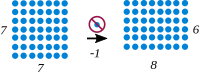
\includegraphics[scale=1.0]{numbersExampleGenerality}
  \caption{49 objects can be arranged in a square 7x7. 48 objects can
    be arranged as a rectangle of 6x8.}
  \label{fig:numbersExampleGenerality}
\end{SCfigure}

An astute farmer notices that 49 sacks of grains can be arranged
in a square with each side having 7 sacks (see the Figure
\ref{fig:numbersExampleGenerality}). When one sack is used up, the
remaining 48 sacks can be arranged as a rectangle 6 by 8 sacks.

The farmer realizes that this curious fact has nothing to do with
either grains or sacks. The same observation could be made about
buckets, chairs, people, and so on. As the first step of
generalization, the farmer states that 49 \emph{objects} can be
arranged as a 7 by 7 square, while 48 objects can be arranged
as a 6 by 8 rectangle. The farmer also notes that $48=49-1$, whereas
$6=7-1$ and $8=7+1$. She writes down the newly discovered relation as
follows:
\begin{align*}
  7*7\textrm{ obj } - 1\textrm{ obj } = (7-1) * (7+1)\textrm{ obj }\,,
\end{align*}
where \emph{obj} is the denotation of \emph{any} object.

As the grain is used up, the farmer discovers two more relations:
\begin{align*}
  6*6\textrm{ obj } - 1\textrm{ obj } = (6-1) * (6+1)\textrm{ obj }
\end{align*}
and
\begin{align*}
  5*5\textrm{ obj } - 1\textrm{ obj } = (5-1) * (5+1)\textrm{ obj }\,.
\end{align*}

At this point the farmer makes an educated guess, stating that a more
general relation must exist:
\begin{align}
  n*n - 1 = (n-1) * (n+1)\,.
  \label{eq:numbersAlgebraIdentity1}
\end{align}
In the last expression the reference to objects is dropped, the
expression is written simply in terms of \emph{numbers}.

A deeper analysis reveals that the relation given by
(\ref{eq:numbersAlgebraIdentity1}) exists for \emph{any quantities}
that obey usual rules of addition and multiplication. This includes
rational numbers, real numbers, complex numbers\index{Numbers!complex} (see Section
\ref{sec:CompoundNumbers}), and even operators! The relation
\begin{align}
  x^2-1=(x-1)(x+1)
\end{align}
 holds true because of the way we define \emph{rules for manipulation} --
 addition and multiplication in this case -- of
number-like objects, regardless of what those number-like objects
represent in a particular problem.
\begin{figure}[htbp]
  \centering
  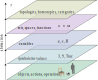
\includegraphics[scale=1.0]{numbersAbstractionLevels}
  \caption{Mathematical thinking has many levels of abstraction\index{Abstraction}. Going
    to higher levels of abstractions results in higher efficiency and
    more powerful ideas and tools.}
  \label{fig:numbersAbstractionLevels}
\end{figure}

The path from ``sacks of grain'' to a variable $x$ is the path from concrete,
specific objects to \emph{abstract} entities that are the product of
creative imagination. This path to higher levels of abstraction is
illustrated in the Figure \ref{fig:numbersAbstractionLevels}. As we
move to higher levels of abstraction, our mathematical tools become
more powerful and more universally applicable: From everyday
arithmetic, to economics, to general relativity, and quantum gravity.

Using more abstract mathematical objects requires serious mental
effort. To reach the highest levels one needs to do mathematics
professionally. However, any profession can benefit from \emph{some} level of
abstraction, and to understand vectors and tensors, we must go beyond
usual high-school level. One of the goals of this book is to help readers
build tolerance and appreciation of more abstract aspects of
mathematics.


\section{Terminology Barrier}
Every high school student has a working knowledge of bilinear operators
over associative and commutative fields\index{Field}, but hardly anyone of those
students is aware of this fact. We refer here to the ability to
simply add and multiply numbers. This demonstrates that even familiar
and basic notions may look complicated when ``dressed in unfamiliar
clothing.''

When we learn new mathematical concepts, especially at a higher level of
abstraction, we often encounter what might be called a
\emph{terminology barrier}\index{Barrier!terminology}: a concept seems
more difficult if it is
formulated in a new language, without sufficient connections to
already familiar concepts, and without clear examples of how the
concept can be applied.

New terminology is unavoidable when learning new concepts. There will
be a number of new mathematical concepts and definition introduced in
this book. To lower the terminology barrier, every new mathematical
concept will be illustrated with examples and the connections to
already familiar concepts will also be given. Additionally, it is
recommended to do the following exercise every time a new concept with
unusual terminology is introduced:

\begin{mybio}{Dealing With New Concepts}
  \begin{itemize}
    \item \phantom{x}
  \item Take a critical look at a new name and notation.
  \item Think whether the new name or notation looks like something
    you know. Is the resemblance helpful or misleading?
  \item Be creative and try to come up with your own notation or word
    to describe the new concept.
  \end{itemize}
  \vspace{0.1cm}
  \emph{Remember}: Symbols and names are not essential. What is
  important is the set of \emph{relations} of a new concept to other
  concepts. The relations show how the concept fits and functions
  within the larger framework.
\end{mybio}
Demonstrations of this approach can be found in the rest of the book.

\section{Algebra of Numbers}

We will start with the ``familiar'' numbers\index{Numbers}:
\begin{align*}
  0,\pm 1, \pm 2, \ldots, \pm n,\,\ldots
\end{align*}
This endless collection, considered as one entity, is called the
\emph{set of whole numbers}; it is denoted as $\mathbb{Z}$.

The set $\mathbb{Z}$ is not a formless heap of elements. On the
contrary, it has a rich \emph{structure}\index{Structure}. The structure of any set, including
the set of whole numbers, is
revealed through various \emph{relations}\index{Relations} between all or some of its
elements. Here are several examples:
\begin{itemize}
  \item $1$ and $-1$ are related, and so are $2$ and
    $-2$, and generally, $n$ and $-n$.
  \item Relation exists between $1$ and $2$, $2$ and $4$, $3$ and $6$,
    and generally, between $n$ and $2n$.
  \item The pairs $(1,2)$, $(2,3)$, $(3, 4$), and so on, illustrate an
    important relation of order that exists in $\mathbb{Z}$.
  \item The pairs $(2, 1)$, $(3, 1)$, $(4, 2)$, $(5, 1)$, $(6, 3)$ and
    similar ones unite a number and its greatest divisor not equal to
    the number itself.
\end{itemize}
The list can be continued indefinitely, but the general idea of
relations should be
clear. Such number-to-number relation can be schematically represented
as a box with an input and an output, as shown in the Figure
\ref{fig:schematicRelation1to1}. A few important relations are given
descriptive names: {\bf neg}, {\bf dbl}, {\bf suc}, and {\bf gsd}
are examples from the Figure \ref{fig:schematicRelation1to1}; they
correspond to negation, doubling of a number, finding the successor of
a given number, and finding the greatest divisor smaller than the
number itself.
\begin{figure}[htbp]
  \centering
  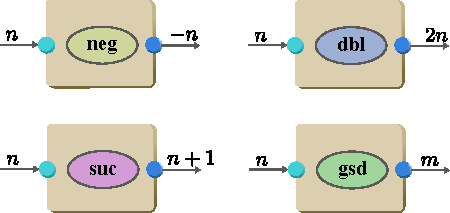
\includegraphics[scale=1.0]{schematicRelation1to1}
  \caption{Relation between elements of a set can be schematically
    represented using boxes with inputs and outputs. Here the
    relations between numbers are given descriptive names: {\bf neg}
    is negation, {\bf dbl} is doubling, {\bf suc} is getting the
    successive number, {\bf gsd} is the greatest divisor of a number smaller than
    the number itself.}
  \label{fig:schematicRelation1to1}
\end{figure}

\subsection{Functions}
What we have just described is the idea of a \emph{function}\index{Function}, or numeric
function of a single \emph{argument}\index{Argument}, to be precise. A function of a
single argument connects every \emph{argument} (input) to a certain
\emph{value} (output), establishing a \emph{relation} between a pair
of elements.
\begin{SCfigure}%[htbp]
  %\centering
  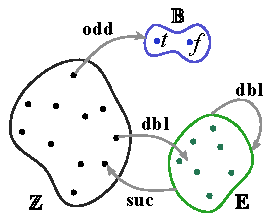
\includegraphics[scale=1.0]{diagramFunctionSingleArg}
  \caption{Relations can be viewed on the level of sets. A function
    maps (connects) one set with another in a meaningful way. For
    example, $\textrm{\bf dbl}$ maps every integer from $\mathbb{Z}$
  into the set of even numbers $\mathbb{E}$.}
  \label{fig:diagramFunctionSingleArg}
\end{SCfigure}

Another view on relations is illustrated in the Figure
\ref{fig:diagramFunctionSingleArg}. Relations between elements can be
``elevated'' to the level of sets and depicted as arrows connecting
one set (\emph{domain}) to another set (\emph{range}). Symbolically we
can write:
\[
\mathbb{Z}\overset{\textrm{\bf dbl}}{\longrightarrow} \mathbb{E}\,,
\]
where $\mathbb{E}$ denotes the set of all even numbers, {\bf dbl} is the
name of the function that doubles its argument.

The relations of the type ``one number to one number'' -- considered
above -- can be
generalized to ``several numbers to one number'' or ``one number to
several numbers'' or even ``several numbers to several numbers.'' The
schematic representation of such relations are given in the
Figure \ref{fig:schematicRelationNtoN}.
\begin{figure}[htbp]
  \centering
  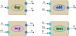
\includegraphics[scale=1.0]{schematicRelationNtoN}
  \caption{Relations of several elements to several elements:
    {\bf dup} duplicates its input, {\bf add} calculates the sum,
    {\bf swp} swaps the order of the arguments, {\bf max} returns the
    maximum of three input numbers.}
  \label{fig:schematicRelationNtoN}
\end{figure}

\begin{exercise}\label{exe:relationsGeneral}
Think how you would represent the generalized relations of the types
given in the Figure \ref{fig:schematicRelationNtoN} at the level of
sets? What kind of diagrams would you draw?
\end{exercise}

\subsubsection{Binary Functions}
An important function of two variables is the familiar {\bf add} relation:
\[
\btc{add}\,n\,m = n + m\,.
\]
The right-hand side of this equality is just another way of writing
the expression involving function with two input arguments. It is a
special case of a more general rule, which can be written as follows:
\[
f\,\,n\,m = n\circledcirc m\,.
\]
On the left we have a \emph{prefix}\index{Notation!prefix} notation, where a function $f$
is \emph{applied} to two arguments. On the right, we have an
\emph{infix}\index{Notation!infix} notation and a special symbol placed between the first
and the second argument. Several familiar examples are:
\begin{itemize}
\item $\btc{mul}\,\,n\,m = n * m$ -- multiplication.
\item $\btc{pow}\,\,n\,m = n^\wedge m$ -- power.
\item $\btc{sub}\,\,n\,m = n - m$ -- subtraction.
\item $\btc{div}\,\,n\,m = n / m$ -- division.
\end{itemize}
The functions $\btc{mul}$, $\btc{pow}$, $\btc{sub}$, and $\btc{div}$ are all examples of
\emph{binary}\index{Function!binary} functions -- functions of two arguments.
\begin{exercise}\label{exe:binaryYourOwn}
Think of a your own example of a binary function (function of two
arguments). Create its infix variant.
\end{exercise}


%\begin{tcolorbox}[colback=white!95!ocre, title=Problem]
\begin{exercise}\label{exe:ESRSymmetricAntisymmetric}
  Show that
  \[
  \epsilon_{ij}a_ia_j = 0\,.
  \]
\end{exercise}
%\end{tcolorbox}

\section*{Chapter Highlights}
{\setstretch{1.5}\chhc
  \it
  \small
\begin{itemize}
\item The power of mathematical concepts and methods increases with
  the level of abstraction.
\item Learning new concepts often involves learning new
  terminology. The latter can create an artificial mental barrier.
\item ``Usual'' numbers form a mathematical structure. The structure
  is revealed through various relations that exist between numbers.
\item Relations between numbers are expressed using the concept of
  functions and operations (e.g., addition). Each operation is
  characterized by its arity -- the number of arguments it accepts as
  an input.
\item Functions can be represented schematically as boxes with inputs
  and outputs.
\item Functions that act on natural numbers can be written using index
  notation (e.g., $f\, i = f_i$).
\item Linear functions represent the simplest but still powerful and
  useful kind of functions.
\item Functions can be composed to create new functions.
\item A function with several inputs is said to be partially applied when not
  all its inputs are populated.
\item The same function can be represented in various ways: Graphical,
  as a symbolic formula, as a table. The function is not reduced to
  any of its representations.
\item The power of abstract mathematical thinking comes, in part, from
  efficient notation. Einstein's Summation Rule (ESR) is a good
  example of this.
\end{itemize}


}

%
%
%%----------------------------------------------------------------------------------------
%%	CHAPTER
%%----------------------------------------------------------------------------------------
%
\chapterimage{pics/chapterImageArrows.pdf}
%\chapterimage{spacetime.pdf}
\graphicspath{{../03Mathematics/pics/}}

\chapter{Mathematics}\label{ch:Mathematics}

\lettrine[lines=2]{\color{darkocre}M}{athematical concepts and tools} used in quantum theory do not differ significantly from the ones used in classical physics.

\begin{myprereq}{Prerequisite Knowledge}
	To fully understand the material of this chapter, readers should be comfortable with the following concepts:
	
	\begin{itemize}
		\item \phantom{phantom}
		\vspace{-0.5cm}
		\item State
		\item Dynamical equations
	\end{itemize}	
\end{myprereq}

\section{Numberlikes}

To arrive at the idea of vectors we will start with simple geometrical
objects -- arrows in a plane, as illustrated in the Figure \ref{fig:arrowsSpace}.


\section{Functions}

To arrive at the idea of vectors we will start with simple geometrical
objects -- arrows in a plane, as illustrated in the Figure \ref{fig:arrowsSpace}.

\subsection{Partial Application}

\subsection{Linearity}

\section{Kalcoolus}

To arrive at the idea of vectors we will start with simple geometrical
objects -- arrows in a plane, as illustrated in the Figure \ref{fig:arrowsSpace}.


\section{Arrows}

To arrive at the idea of vectors we will start with simple geometrical
objects -- arrows in a plane, as illustrated in the Figure \ref{fig:arrowsSpace}.

\begin{figure}[htbp]
  \centering
  
\includegraphics[scale=1.0]{defaultFigureTemplate}
  \caption{Set of arrows starting at the same origin point $O$. All
    imaginable arrows taken as one set form the arrow space
    $\overset{\Rightarrow}{A}$.}
  \label{fig:arrowsSpace}
\end{figure}

Symbolically, we will denote vectors by placing an arrow over letters:
\[
\vec{a}\,,\vec{b}\,,\vec{c}\,,\ldots\,,\vec{\alpha}\,,\vec{\beta}\,.
\]

\subsection{Dirac Notation}

\section{Scalar Product}

To arrive at the idea of vectors we will start with simple geometrical
objects -- arrows in a plane, as illustrated in the Figure \ref{fig:arrowsSpace}.


\section{Operators}

To arrive at the idea of vectors we will start with simple geometrical
objects -- arrows in a plane.
\[
\braket{\phi}{\phi}
\]
and
\[
\ketbra{\phi}{\phi}\,.
\]

\subsection{Super-operators}

An action of an operator $F$ on arrows can be represented symbolically
as an equation:
\[
F\,\vec{a}=\vec{b}\:.
\]
Often a ``hat'' is placed on top of an operator\footnote{In Quantum
	Mechanics, for example.}, to emphasize that it is different from
numeric function:
\[
\colorboxed{red}{
	\op{F}\,\vec{a}=\vec{b}\:.
}
\]

\begin{mybio}{Simple Operators}\\
	It is easy to come up with examples of operators:
	
	\begin{itemize}
		\item\phantom{x}
		
		\item Unit operator (or \emph{identity} operator), such that
		\[
		\op{I}\,\vec{a}=\vec{a}\,.
		\]
		
		\item ``Zeroing'' operator that maps every vector into a zero
		vector:
		\[
		\op{0}\, \vec{a} = \vec{0}\,.
		\]
		
	\end{itemize}
\end{mybio}


To fully describe an operator, we must describe how it acts \emph{on
	every} arrow. 

\begin{flushleft}
	{\bf Examples}
\end{flushleft}
Let us take a closer look at a couple of operators. While studying
these examples we must keep in mind that the relations between
components are \emph{specific to basis} and will change if we change the
basis. The question of how exactly the relation between components
changes will be addressed later in Section
\ref{sec:ComponentTransformation} for the simplest types of operators.


\begin{mybio}{Matrix}
	Here is an example of matrix:
	\[
	\op{S} =
	\begin{pmatrix}
		S_{11} & S_{12}\\
		S_{21} & S_{22}
	\end{pmatrix} =
	\begin{pmatrix}
		\alpha & 0\\
		0 & \alpha
	\end{pmatrix}\,.
	\]
	Similar approach can be used to find the components of any linear operator.
\end{mybio}


\section{Functionals}
Another important type of function is called \emph{functional}. A functional maps a function into a number. Let's consider several examples.

\subsection*{Total Mass}
Suppose an astrophysicist is trying to model a spherically symmetric star and calculates \emph{density} of the star as the function of distance from its center: $r\rightarrow\rho_r$. The total mass of the star can then be evaluated as the sum of masses of all spherical shells with thickness $\delta r$:
\[
M = \int \delta V\rho_r=\int 4\pi r^2\delta r\rho_r\,.
\]
For a given function $\rho_r$ this summation will result in a number -- star's total mass. Such mapping $\rho_r\rightarrow M$ is an example of a functional.

\subsection*{Total Fuel}
Consider a car moving on a straight highway between two points $A$ and $B$. The amount of fuel the engine consumes at a given moment depends on the speed of the car at that moment and can be described by the function $\mu_v$. Suppose the position of the car as the function of time $x_t$ is known and are looking for the total fuel consumed during the travel. This can be done in three steps. 

First, we find the speed of the car as the function of time by applying the operator $\partial_t$ to $x_t$: $v_t=\partial_{t}x$. Second, we find the fuel consuption rate $\mu$  as the function of time by plugging $v_t$ into $\mu_v$: $f_t = \mu(v_t)$. Finally, we can find the total amount of consumed fuel as the sum
\[
F = \int f_t\delta t\,.
\]
Combining all three steps into a single mathematical expression will result in a more cumbersome formula:
\[
F = \int \delta t\mu(\partial_t x)\,.
\]
This formula encodes a recipe for mapping any function $x_t$ into a number $F$ -- an example of a functional.

\subsection*{Total Action}
A body in a "freely fall" is moving with constant acceleration due to the force of gravity. Its speed increases as the body approaches the ground. If the body starts at rest at height $H$, its position along the vertical $y$ axis depends on time as $y_t=H-gt^2/2$ and the velocity changes according to the equation $v=-gt$.

The potenital energy $E_p=mgy$ of the body decreases, while its kinetic energy $E_k=mv^2/2$ grows. The total mechanical energy $E=E_p+E_k$ remains fixed according to the law of energy conservation. Thus, the potential energy of the body is transformed into the kinetic energy.

Another physical quantity is often important -- the \emph{imbalance} of kinetic energy over the potential energy:
\[
L = E_k - E_p\,.
\]
It does not remain constant, and for the case of a free fall we can easily find its time dependence:
\[
L_t = mg^2t^2 - mgH\,.
\]
Given $L_t$, we can calculate a fundamental physical quantity -- total \emph{action} of the process:
\[
A = \int\delta t L_t\,.
\]
The summation extends to the moment $t=T$ when the body reaches the ground ($y=0$). This happens at $T=\sqrt{2H/g}$.

Performing the summation requires evaluation of two familiar sums:
\[
\int t^2\delta t =\frac{T^3}{3}\quad\textrm{ and }\quad \int \delta t=T\,.
\]
Substituting the values of $T$ and simplifying, the expression for the total action takes the form
\[
A = mgT(\frac{gT^2}{3}-H)=-\frac{mH}{3}\sqrt{2gH}=-\frac{mv_{m}H}{3}\,.
\]
Here we used $v_m=gT=\sqrt{2Hg}$ -- the maximal speed of the body at the end of the free fall process. Finally, denoting the maximum momentum of the body as $p_m=mv_m$, we obtain $A=-p_m H/3$. Note that the action can be expressed as the product of momentum and distance.

\emph{Action} is a physical quantit of fundamental importance. It plays a prominent role in both classical mechanics (the principle of \emph{stationary action}) and in quantum physics (the principle of \emph{action quantization}). Both principles will be explored in details later in the book.

\begin{exercise}
	Calculate the total action of a free fall process for an electron falling from the height 0.1 meter.
\end{exercise}



\subsection*{Assorted Examples}
Examples of functionals given above involve evaluation of sums in order to find  \emph{total quantities} of various kinds:
\[
Q = \int \delta x f_x\,.
\]
The total quantity $Q$ depends on the behavior of the input function $f_x$ over an extended range of $x$ values. Simpler forms of functionals can also be used. For example:
\[
\mathcal{M}\, f = f_0
\]
returns the value of the input function $f_x$ at zero. This functional, despite its trivial look, is very useful and widely used in physics and mathematics. Its rigorous mathematical form is called \emph{Dirac delta function}\,.
\begin{mybio}{Dirac Delta Function}
	The idea of delta function is simple: it describes the density of mass (or charge, probability, and so on) for a point-like particle. Formally, such density can be written as $\delta_x$.
	
	Since the total mass (charge, probability) is finite, the summation of the density over the region where the particle might be must be a fixed number:
	\[
	m = \int \delta x \delta_x\,.
	\]
\end{mybio}

Another example of a simple functional is the maximum of a function:
\[
\mathcal{X}\,f = \textrm{max}\,f_x\,.
\]
Finally, one can map any function $f_x$ into a number like so:
\[
\mathcal{R}\,f = \frac{f_1}{1!} + \frac{f_{1/2}}{2!} + \frac{f_{1/3}}{3!}+\ldots+\frac{f_{1/n}}{n!}+\ldots\,.
\]
For $f=\sin$ we obtain $\mathcal{R}\,\sin\approx 1.1479$.
\begin{exercise}
	For the functionals $\mathcal{M}$, $\mathcal{X}$, and $\mathcal{R}$ check whether they are \emph{linear}.
\end{exercise}

\section{Spaces}

To arrive at the idea of vectors we will start with simple geometrical
objects -- arrows in a plane.
\[
\braket{\phi}{\phi}
\]
and
\[
\ketbra{\phi}{\phi}\,.
\]

\section{Application: Circular Motion}
Let us examine how the concepts and tools discussed above can be applied to a simple case of circular motion.  

Consider a  particle moving in a circle with the radius $R$, as shown in Figure X. If we choose the center of the circle as the reference point, we can specify the position of the particle using an arrow $\ket{r}$. During motion the direction of this arrow is constantly changing, but its length $R$ remains the same.  

After a short time interval $\delta t$, the position of the particle changes by $\delta\ket{r}$:
\[
\ket{r_t}\quad\rightarrow\quad \ket{r_{t+\delta t}} = \ket{r_t}+\delta\ket{r}\,.
\]

The length of the path covered by the particle during the time interval $\delta t$ can be approximated by the length of the arc  $\delta L=R\delta\theta=v\delta t$. The arrow $\delta\ket{r}$ can be written as $\delta L\ket{u}$ where $\ket{u}$ is the vector of unit length pointing in the direction of motion. This unit vector can be constructed from $\ket{r}$ by scaling it down by $R$ and then rotating counter-clockwise with the operator $\op{J}$: 
\[
\delta\ket{r}=R\delta\theta\op{J}\left(\frac{\ket{r}}{R}\right)\,.
\]
Since $\op{J}$ is a linear operator, the $R$ cancels and we can write
\[
\frac{\delta\ket{r}}{\delta t}=\frac{\delta\theta}{\delta t}\op{J}\ket{r}\qquad\Longrightarrow\qquad
\partial_t\ket{r}=\omega\op{J}\ket{r}\,,
\]
where we introduced the angular speed $\omega=\partial_t\theta$. Finally, by applying the $\op{J}$ operator to both sides of the last equation, we can cast it into the "Schrodinger" form:
\[
\op{J}\partial_t\ket{r}=-\omega\ket{r}\,.
\]  



\section*{Chapter Highlights}
{\setstretch{1.5}\chhc
  \it
\begin{itemize}
\item Arrows in a plane provide a simple model for vectors.
\item Arrows can be manipulated in ways analogous to numbers: Two arrows
  be added, an arrow can be ``scaled'' (stretched or compressed). Arrows form
  an algebra.
\item Basis is an extremely important concept. Basis is a set of
  objects (arrows) that can be used to ``build'' all other similar
  objects (arrows). At the same time, basis can not be used to build
  itself -- basis arrows are independent.
\end{itemize}
}

%

%----------------------------------------------------------------------------------------
%	PART
%----------------------------------------------------------------------------------------
%\part{Part B}

\chapterimage{pics/chapterImageOperators.pdf}
\graphicspath{{../04ClassicalPhysics/pics/}}

\chapter{Classical Physics}\label{ch:ClassicalPhysics}
\begin{quoting}
	I think we may ultimately reach the stage when
	it is possible to set up quantum theory without any reference to classical theory,
	just as we already have reached the stage where we can set up the Einstein
	gravitational theory without any reference to the Newtonian theory. But
	from the point of view of teaching students, I think one would always
	have to proceed by stages -- not expect too much from them, teach them
	first the elementary theories and gradually develop their minds; and
	that will always involve working from the classical theory
	first.
	
	P. A. M. Dirac, Lectures on Quantum Field Theory, Belfer Graduate
	School of Science, Yeshiva University, New York, 1966, p.43.
\end{quoting}

\lettrine[lines=2]{\color{darkocre}T}{he} concept of
\emph{operators}\index{Operator} extends the idea of functions. An unary numeric
function $f$ takes some numeric value $x$ as an input  and produces
another numeric value $y$:
\[
f\,x=y\quad \textrm{ or } \quad x\overset{f}{\longrightarrow} y\,.
\]
In mathematical jargon, $f$ \emph{maps} $x$ into $y$.

\begin{myprereq}{Prerequisite Knowledge}
	To fully understand the material of this chapter, readers should be comfortable with the following concepts:
	
	\begin{itemize}
		\item \phantom{phantom}
		\vspace{-0.5cm}
		\item State
		\item Dynamical equations
	\end{itemize}	
\end{myprereq}


\begin{figure}[htbp]
  \centering
  
\includegraphics[scale=1.0]{defaultFigureTemplate}
  \caption{Operators extend the idea of functions. (a) An unary
    function $f$ can be applied to a number $x$ to produce
    another number $y$. (b) An unary operator $\op{F}$ can be applied to a vector
    $\vec{a}$ to yield another vector $\vec{b}$.}
  \label{fig:arrowsOperatorGeneral}
\end{figure}

\section{System}\label{sec:System}
A part of nature that can be clearly isolated and studied is called a \emph{physical system}. An electron, an atom, a molecule, a crystal, a pendulum, a comet, a star – these are examples of physical systems of various degrees of complexity.

Often a physical system is a body or several bodies interacting with each other or with some external bodies. Figure \ref{fig:systemExamples} provides several examples of \emph{mechanical systems}. Let’s examine them in more detail.
\begin{figure}[htbp]
	\centering
	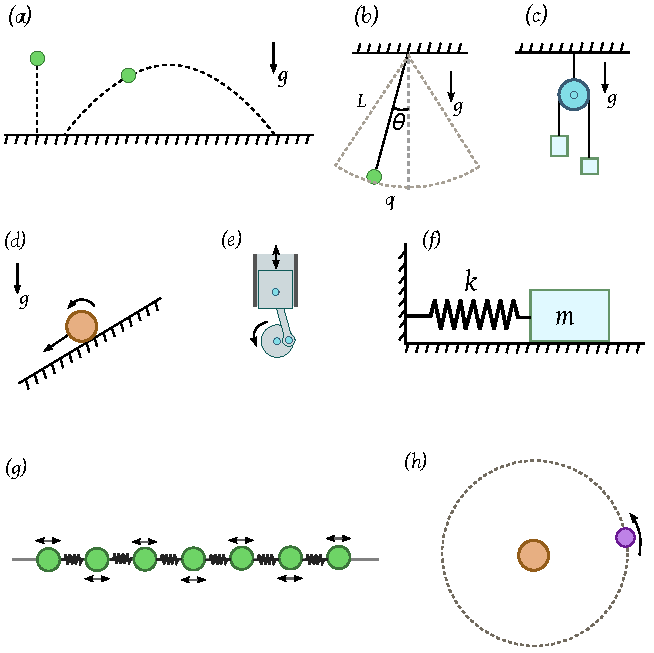
\includegraphics[scale=1.0]{systemExamples}
	\caption{Examples of mechanical systems. See text for explanation..}
	\label{fig:systemExamples}
\end{figure}
\renewcommand{\labelenumi}{(\alph{enumi})}
\begin{enumerate}
	\item \emph{Free falling body}: An elastic body falls down vertically under the
	force of gravity, bounces back, goes up and then down to repeat the
	bounce again and again. Also, a projectile launched at an angle.
	\item \emph{String pendulum}: A compact body is attached to a string
	of fixed length. It is allowed to swing back and forth without
	experiencing air friction.
	\item \emph{Atwood machine}: Two bodies with slightly unequal masses
	are connected with a non-stretchable string going over a
	frictionless pulley.
	\item \emph{Inclined plane}: A solid cylinder rolling down an
	inclinded plane.
	\item \emph{Piston}: A system of three bodies (cylindrical
	crankshaft, rod, and piston) connected in a way that locks rotation
	of a cylinder and the vertical motion of the piston.
	\item \emph{Spring oscillator}: A body, attached to a spring, is
	allowed to slide left and right across a frictionless surface.
	\item \emph{Linear chain of oscillators}: A set of pairwise
	interconnected identical bodies; the allowed motion happens along
	the horizontal axis.
	\item \emph{Sun and planet}: A planet circling around the sun.
	
\end{enumerate}
We will study oscillator and circular motion in great detail.

\subsection{Configuration}
In mechanics, \emph{configuration} means a formal way to describe the
arrangement of a system at a given time.

The behavior of a system in time can be described by specifying its
\emph{configuration} as the function of time. In relatively simple
systems, configuration may consist of a set of coordinates that uniquely
determine the arrangement of bodies in the system. For example, the
configuration of a pendulum can be given by a single coordinate --- the
length of the arc $q$. Of course, as the pendulum swings, both
Cartesian coordinates $x$ and $y$ are changing, but not independently,
due to the relation
\begin{equation*}
	x^2 + y^2 = L^2\, .
\end{equation*}
Given $x$, we can find $y > 0$ as $y = +\sqrt{L^2 - x^2}$, thus
reducing the number of required coordinates.

Consider another example, shown in the Figure
(\ref{fig:coupledSystem})(a): a system of
two bodies, connected with each other using ideal springs with
stiffness $k$, and each body is connected to a rigid wall.
\begin{figure}[htbp]
	\centering
	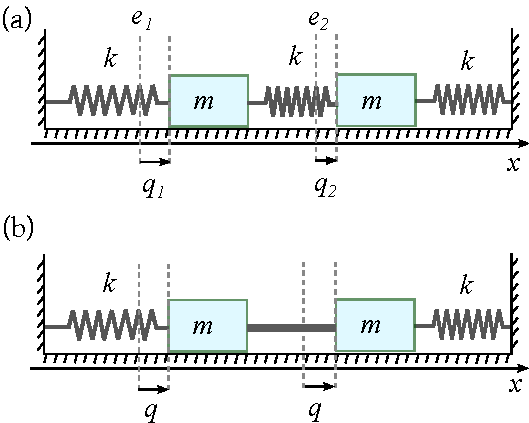
\includegraphics[scale=1.0]{coupledSystem}
	\caption{(a); (b).}
	\label{fig:coupledSystem}
\end{figure}

When the system is in equilibrium, the bodies occupy positions on the
horizotal axis denoted as $e_1$ and $e_2$. During motion, the position
of the first body changes by
\begin{equation*}
	q_1(t) = x_1(t) - e_1\, ,
\end{equation*}
and similarly for the second body: $q_2 = x_2 - e_2$. It is important
to realize, that although the two bodies are connected with a spring,
they can still move with different velocities, and have different
displacements $q_1 \ne q_2$. Indeed, we can set the system in motion
by moving each body independently and then releasing them. Contrast
this with the situation, shown in the Figure
(\ref{fig:coupledSystem})(b), where the bodies are connected with a
rigid rod, fusing two masses into essentially a single body. In this
case only a single displacement $q$ is required to specify the
configuration of the system.

\subsection{Qoordinates}
The coordinates specifying the configuration of a system do not
have to be Cartesian. In the example of a pendulum, the configuration
can be conveniently given by the length of the arc $q=L\theta$, see
Figure (\ref{fig:systemExamples})(b).

Consider another example, shown in the Figure
(\ref{fig:systemExamples})(h): Two bodies interact
gravitationally. In this problem, it turns out, the equations
describing the motion of the system are simpler if, instead of the
usual positions $x_1$ and $x_2$ we use the relative distance
\begin{equation*}
	q_1 = x_2 - x_1
\end{equation*}
and the position of the center of mass
\begin{equation*}
	q_2 = (m_1x_1 + m_2x_2)/(m_1 + m_2),
\end{equation*}
where $m_1$ and $m_2$ are the masses of the bodies.

We thus come to the idea of \emph{generalized coordinates} --
arbitrary coordinates completely specifying the configuration of a
system. Generalized coordinates can be based on positions, angles, or
some combinations of those.

\subsection{Degrees of Freedom}
\emph{Degree of freedom} is a separate independent motion of a
mechanical system. Each independent motion corresponds to the change
in time
of a separate generalized coordinate. The number of degrees of freedom
is the number of
generalized coordinates required to completely specify the
configuration of a mechanical system at different moments of time.

Take, for example, a pendulum, shown in the Figure
(\ref{fig:degreeOfFreedomPendulum}). In general Cartesian coordinates,
all three coordinates $x$, $y$, and $z$ will be changing in
time. However, only a single generalized coordinate $q(t)$ --- the
length of the arc -- is required to fully describe the configuration,
and thus the motion, of this mechanical system. The number of degrees
of freedom, in this example, equals 1.

\begin{figure}[htbp]
	\centering
	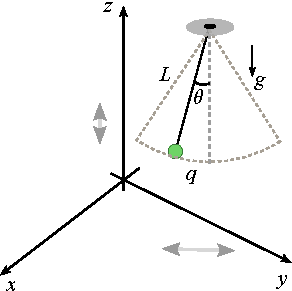
\includegraphics[scale=1.0]{degreeOfFreedomPendulum}
	\caption{A pendulum has one degree of freedom, despite the fact
		that all three Cartesian coordinates can be changing during its motion.}
	\label{fig:degreeOfFreedomPendulum}
\end{figure}




\section{Oscillator}\label{sec:Oscillator}
The model of an oscillator is extremely important. It appears in
various guises in almost all physical theories. Let's study it in details.

\begin{figure}[htbp]
	\centering
	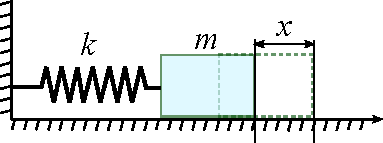
\includegraphics[scale=0.9]{Oscillator}
	\caption{A mechanical model of an oscillator: A body attached to an
		ideal spring.}
	\label{fig:Oscillator}
\end{figure}


Consider a body with the mass $m$ is attached to a spring with the stiffness
$k$. The body is allowed to move across a frictionless
surface.  The force required to strech a spring by the amount $x$
is given by the Hooke's law
\[
F=kx.
\]
This is the force applied \emph{to the spring}. The force created
\emph{by the spring, and applied to the attached body}, is of equal
magnitude but points in the opposite direction.

When the body is displaced from its equilibrium position,
by stretching or compressing the spring, and then released, it will
undergo periodic motion. During this motion, the position, velocity,
kinetic energy of the mody, and the potential energy of the spring
will be constantly changing.

To remind, the kinetic energy of a body is

\[
E_{k}=\frac{mv^{2}}{2}, \textrm{ or } K = \frac{p^2}{2m}\,.
\]
The potential energy of a spring, stretched or compressed by the
amount $x$ is given by

\[
E_{p}=\frac{kx^{2}}{2}, \textrm{ or } \Pi = \frac{kq^2}{2}\,.
\]


\section{State}\label{sec:State}
\emph{State} of a system is the \emph{minimal} collection of observables which is, in
certain sense, \emph{complete} and \emph{self-sufficient}. State is 
"all there is to know" about a system. If the state of a system is known at one
moment of time $t_0$, then we should be able to determine the state
at any later moment of time $t$. In classical mechanics the pair of
observables $(x, p)$ defines the state of a mechanical system.

\emph{State} is the minimal set of quantities describing mechanical
system and sufficient to predict
their future values from their initial values. State is an important
concept not only mechanics, but in other areas of physics.
Let's elaborate, using the oscillator as an example.

Suppose that at the moment of time $t_{0}$ the position of an oscillator
is $x_{0}$ and its velocity is $v_{0}$. To find their values at
some later time $t>t_{0}$, we can go iteratively in small steps, calculating
how much the position and the velocity change after each successive
tiny interval of time $\delta t$. The first iteration results in
the updated value of position
\[
	x_{1}=x_{0}+v_{0}\delta t.
\]
The second, and every other, iteration looks very similar:
\[
	x_{2}=x_{1}+v\delta t\,.
\]
Now it is important to realize that we can no longer use the same initial
velocity $v_{0}$ in the second iteration, because the velocity itself
changes. Thus, we must update the value of the velocity as well. This
is done by using acceleration:
\[
	v_{1}=v_{0}+a_{0}\,.
\]
After that, we can find the second iteration of the position:
$x_{2}=x_{1}+v_{1}\delta t$. To keep this scheme going, we must be
able to update the value of the acceleration, because it is also changing.
It appears then, we need some quantity that allows to find the next
step:
\[
	a_{1}=a_{0}+b_{0}\delta t\,.
\]
Fortunately, \emph{this is not needed!} At this point we can use the laws of motion.
For example, Newton's second law gives the acceleration in terms of the known force acting on the object:
\begin{equation}
	a=\frac{F}{m}.
\end{equation}
{\it Forces don't depend on acceleration}

All known forces in physics depend on positions or distances and--
sometimes-- velocities of bodies. For example, the force of the spring $F=-kx$
depends only on the coordinate $x$. The force of gravitational interaction $F=GMm/r^2$
and the Coulomb force between two charges $F=kQq/r^2$ depend on the distance
$r$ between the bodies. The force acting on an electron moving through
a magnetic field--known as Lorentz force\index{Lorentz!force}-- equals $F=qvB$ and 
depends on the electron's velocity (and the field's strength $B$). 
No known forces depend on acceleration. This fact leads to an important conclusion:
It is enough to know position and velocity of an object at time $t_{0}$,
in order to find their values at any later moment of time $t>t_{0}$.
Obviously, position and velocity at any previous moment of time can
be found in the similar way.

Thus, we do not need to advance the acceleration by calculating its
small change $\delta a=b\delta t$, we can simply calculate it from
the law of motion:
\begin{equation}
	a_{n}=\frac{F(x_{n},v_{n})}{m}\,.
\end{equation}

This formula says that the acceleration at the iteration step number
$n$ is found from the values of the position $x_{n}$ and the velocity
$v_{n}$ at the same step. Given the velocity, we can advance the
postion, and given the acceleration, we can advance the velocity.
Then we recalculate the new value for the acceleration and repeat,
until we reach the final time $t$.

The preceding discussion demonstrates that in Newtonian mechanics
\emph{the state of a mechanical system} is given by a pair of quantities
-- $(x,v)$. There are alternatives to the Newtonian mechanics, and,
correspondingly, there are alternatives to the mechanical state. The
first such alternative is Hamiltonian dynamics.

\subsection{State Evolution: Newtonian Approach}
We will now apply the ideas and formulas of Newtonian mechanics to an
oscillator. We will calculate the motion of the oscillator in time
using a simple method of \emph{state evolution}. Specifically, we will
setup two simple equations -- one for position and one for velocity.

The equation for position is trivial and amounts to the definition:
\[
\frac{\delta x}{\delta t} = v\,.
\]
The equation for velocity follows from the second law of Newtonian
dynamics:
\[
\frac{\delta v}{\delta t} = \frac{F}{m} = -\frac{kx}{m}\,.
\]
Here we used the expression for the spring force $F=-kx$ acting
\emph{on the body} from the side of the spring.

Suppose we know the \emph{initial state} of the oscillator
$(x_0, v_0)$ at time $t_0=0$. When the clock makes a single tick after
a tiny time interval $\delta t$ the body will move to a new position
\[
x_1 = x_0 + v_0\delta t
\]
and the velocity will change due to the action of the spring:
\[
v_1 = v_0 -\frac{kx_0}{m}\,.
\]
Thus, after a single tick of the clock the state of the oscillator
will evolve from $\ket{\xi}_0=(x_0, v_0)$ to $\ket{\xi}_1=(x_1, v_1)$. At this point we can
keep repeating the steps to calculate the state after any number of
ticks, up to the desired time $t=N\delta t$.

We can now formalize the recipe for evolution of the state, writing it as a mathematical relation:
\[
\ket{\xi}_{new} = f\,\ket{\xi}_{old}\,,
\]
where 
\[
\ket{\xi}_{new}=(x_{new}, v_{new}) = (x_{old}+v_{old}\delta t, v_{old} - kx_{old}/m)\,.
\]
\begin{figure}[htbp]
	\centering
	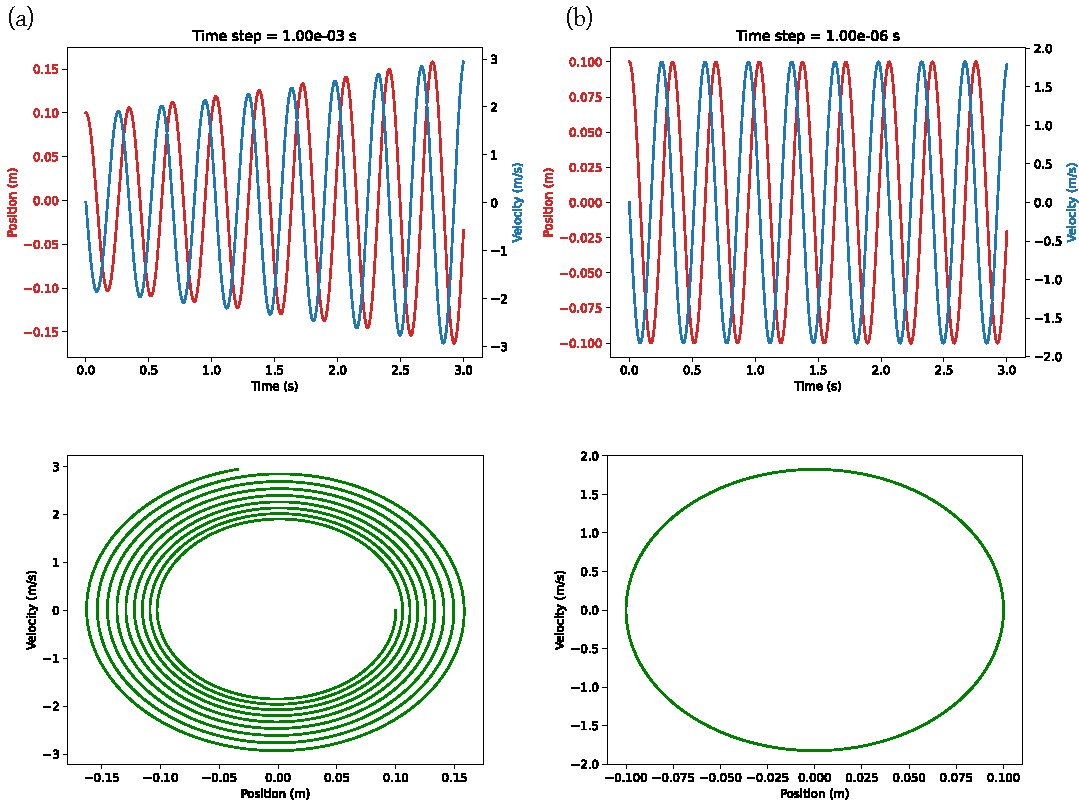
\includegraphics[scale=0.65]{newtonianStateEvolution}
	\caption{First row: Position (red curve, left axis) and velocity (blue
		curve, right axis) as functions of time. Second row: Velocity vs position.
		(a) Calculations with time step of 1 millisecond. (b) Calculations
		with time step of 1 microsecond.}
	\label{fig:newtonianStateEvolution}
\end{figure}

Using this simple approach, we can calculate the state $\ket{\xi}=(x, v)$ of the
oscillator for any moment in the future or past. Figure
\ref{fig:newtonianStateEvolution} shows two example results. The first
result, in the column (a), demonstrates that we must be careful with
the step size $\delta t$ of the time. If it is not sufficiently small,
the inherent error of the method accumulates quickly, resulting in
wrong behavior, such as the gradual increase of velocity and
oscillation amplitude. The column (b) of Figure
\ref{fig:newtonianStateEvolution} demonstrates the expected behavior
of the oscillator -- periodic change of position and velocity with constant amplitudes.

\section{Dynamics}\label{sec:Dynamics}
\emph{Dynamics} is the study of state evolution of various systems subject to known interactions. 
Physical systems of interest can be mechanical, like the ones given in example above (WHERE? REF), or  "non-mechanical" like electromagnetic field or even gravitational field. One can also explore dynamics of quantum systems.
 
The central equation in dynamics describes the state change in time due to known \emph{laws of dynamics}:
\[
\partial_t\,\ket{\xi}=\op{D}_{int}\,\ket{\xi}\,.
\]
We will explore three main variants of classical dynamics: Newtonian, Hamiltonian, and Lagrangian. They will prepare us for better understanding \emph{quantum dynamics}.

Newtonian dynamics is based on the notion of \emph{force} as the driver of interaction:
\[
(\partial_t\,x,\,\partial_t\, v)=(v, F/m)\,.
\]
Both Hamiltonian and Lagrangian mechanics rely on the notion of energy. 

\section{Hamiltonian}\label{sec:Hamiltonian}
\emph{Hamiltonian} is the expression for total energy of a system in terms of position and momentum. For example, using the non-relativistic expression for momentum $p=mv$, the Hamiltonian of  an oscillator can be written as
\begin{equation}
	H = \frac{p^2}{2m} + \frac{kx^2}{2}\,.
	\label{eq:OscillatorHamiltonian}
\end{equation}

Hamiltonian, denoted simply as $H$, still means the total energy. The only difference between $H$ and $E$  is the emphasis on the use of momentum in $H$ instead of velocity.

{\it Momentum is more fundamental than velocity.}

Although velocity feels more intuitive and closer related to our visual perception of motion, momentum is a more \emph{fundamental quantity} in physics. There is a \emph{conservation of energy and momentum} law, but there is no law of the conservation of velocity.

\subsection{Phase Space}
Hamiltonian dynamics uses position $x$  and momentum $p$  to study motion. For an isolated system with conserved energy (constant Hamiltonian), the expression for the Hamiltonian establishes the relationship between $x$ and $p$  for all moments of time. For example, using the Hamiltonian for an oscillator (\ref{eq:OscillatorHamiltonian}), we can rewrite it as follows:
\begin{equation}
	1=\frac{p^2}{(2mH)}+\frac{x^2}{(2H/k)}\,.
	\label{eq:phaseSpaceEllipse}
\end{equation}
This has the same form as the equation of an ellipse in Cartesian axes $(x,y)$:
\[
1=\frac{y^2}{b^2}+\frac{x^2}{a^2}\,.
\]
The area of such an ellipse with the semi-axes $a$ and $b$ is $A=\pi ab$. For $a=b$ an ellipse becomes a circle with the area $A=\pi R^2$.

The equation (\ref{eq:phaseSpaceEllipse}) describes an ellipse in a special $xp$-plane, every point of which can be specified by a pair of values $(x,p)$. Such a plane is called \emph{phase space}. It plays an important role in Hamiltonian dynamics.

The maximum value of the momentum is $p_{max}=\sqrt{2mH}$ and the maximum value for the displacement of the body is $x_{max}=\sqrt{2H/k}$. It turns out, the \emph{area of the ellipse in the phase space is directly proportional to the total energy of the oscillator}:
\[
A=\pi x_{max}p_{max}=2\pi H\sqrt{m/k}\,,
\] 
or
\[
H=\frac{A}{2\pi}\sqrt{\frac{k}{m}}\,.
\]
This important relationship will be used later when we will study quantum properties of the oscillator.

\subsection{Hamiltonian Equations}
Hamiltonian dynamics tracks the time dependence of position $x_t$ and momentum $p_t$. The pair of values $(x,p)$ represents the \emph{state in Hamiltonian dynamics}. Indeed, since there is a unique relationship between the momentum and velocity (e.g. $p=mv$ for non-relativistic speeds $v\ll c$, $c$ — speed of light), the knowledge of $\ket{\xi}=(x,p)$ is equivalent to  the knowledge of $\ket{\xi}=(x,v)$ which is the state in Newtonian dynamics. Put differently, the pair $(x,p)$ provides the same complete description of the system as $(x, v)$.

The main difference between Newtonian and Hamiltonian approaches, is that in the latter the equations for the rate of change of $x$ and $p$ are \emph{explicitly tied to the Hamiltonian}— to the form of the energy expressed in terms of position and momentum. In other words, the equations for $\partial_t\,x$ and $\partial_t\,p$ are written in the following  form:
\[
\partial_t\, x = \op{X}\,H\,\quad\textrm{ and }\quad \partial_t\, p = \op{P}\,H\,.
\]
where $\op{X}$ and $\op{P}$ are some \emph{rules} for calculating velocity $v=\partial_t\, x$  and force $F=\partial_t\,p$ from Hamiltonian $H$. Mathematically, $\op{X}$ and $\op{P}$ must be \emph{operators}: they take the function $H(x,p)$ and calculate the functions $v(x,p)$ and $F(x,p)$.

Let’s use the oscillator model to see how exactly these equations look like. 

\begin{exercise}
	Show that for an oscillator $v=p/m=\partial_p\, H$ and $F=-kx=-\partial_x\, H$.
\end{exercise}
Using the results of the exercise, we can conclude that for the oscillator the equations of Hamiltonian dynamics are
\begin{align}
	\label{eq:HamiltonianEquationsA}
	\partial_t\,x & =  \partial_p\, H\,,\\
	\partial_t\,p & = -\partial_x\, H\,. 
	\label{eq:HamiltonianEquationsB}
\end{align}
The equations (\ref{eq:HamiltonianEquationsA}) and (\ref{eq:HamiltonianEquationsB}) are called \emph{Hamiltonian equations of motion}.

\begin{exercise}
	In special theory of relativity it is shown that the energy $E$ and momentum $p$ of any particle are related to its mass $m$ as follows:
	\[
	m^2=E^2-p^2\,.
	\]
	(Special units must be used for this equation to hold. In these special units all velocities are measured as the fractions of the speed of light, while energy, momentum, and mass are all measured in the same units.)
	
	Starting from the Hamiltonian of a relativistic particle 
	\[
	H^2=p^2+m^2\,,
	\]
	show that the momentum depends on velocity as
	\[
	p=\frac{mv}{\sqrt{1-v^2}}\,.
	\]
	Then show that momentum and energy are related as $p=Ev$.
\end{exercise}

\subsection{Solving Oscillator Equations}
We will now find the exact time dependence of both position $x_t$ and momentum $p_t$ of the oscillator. To do that, we will need to take another look at the evolution of the state of the oscillator in phase space.

The state of an oscillator corresponds to a point in the phase space. This point can be mathematically represented either as a vector $\ket{\xi}$ connecting the origin and the point, or as a pair of values $(x,p)$ . Two descriptions are equally valid. Moreover, the pair of values $(x,p)$  can be considered as the components of the vector $\ket{\xi}$. 

As the time progresses, the position and momentum of the oscillator change, but the tip of the arrow $\ket{\xi}$ remains on the ellipse, corresponding to a constant energy $H$. The axes of "ordinary" phase space have different physical units, whereas the "usual" Cartesian axes $(x,y)$ have the same units and are equivalent in their meaning. It is convenient to temporarily introduce \emph{normalized} energy, position, and momentum.

First, let us express the energy of the oscillator in terms of the rest-energy of the electron $E_e=m_e c^2$. Then the Hamiltonian of the oscillator (its total energy) can be written as $H=\bar{H}E_e$. If the rest-energy and Hamiltonian are measured in Joules, then $\bar{H}$ is a number without units. (COOKIES?)

\section{Lagrangian}\label{sec:Lagrangian}
State is $\ket{\xi}=(q, u)$ where $q$ is the generalized coordinate and $u=\partial_t\, q$ is \emph{generalized velocity}.
Generalized momentum:
\[
\pi = \partial_u\,L\,,
\]
Euler-Lagrange equation:
\[
\partial_t\,\pi = \partial_q\,L\,.
\]

\section{Field}\label{sec:Field}
In physics, \emph{field} is a \emph{dynamical system} with infinite number of degrees of freedom. It's dynamics can be studied using either Lagrangian or Hamiltonian approach.

\section{Ideal Versus Real}\label{sec:IdealVsReal}
An action of an operator $F$ on arrows can be represented symbolically
as an equation.



\section*{Chapter Highlights}
{\setstretch{1.5}\chhc
  \it  
\begin{itemize}
\item Operators extends the idea of functions.
\item Numeric functions (e.g., $\sin\,x$) act on numbers and yield
  other numbers. Operators may act on vectors to yield other vectors
  or numbers.
\item Linear operators represent the simplest and yet powerful class
  of operators on vectors.
\item Linear operators can be represented graphically or symbolically.
\end{itemize}

}
%


%----------------------------------------------------------------------------------------
%	PART
%----------------------------------------------------------------------------------------
%\part{Part C}
%\chapterimage{relativity.pdf}
\chapterimage{pics/chapterImageTensors.pdf}
\graphicspath{{../05QuantumPhysics/pics/}}

\chapter{Quantum Physics}\label{ch:QuantumPhysics}
\lettrine[lines=2]{\color{darkocre}T}{he} first type of operators -- and
corresponding tensors -- that we encountered has a simple type:
\[
\op{L}\,\vec{a} = \vec{b}\,.
\]
It is a linear unary function mapping vectors into vectors.


\begin{myprereq}{Prerequisite Knowledge}
To fully understand the material of this chapter, readers should be comfortable with the following concepts:

\begin{itemize}
	\item \phantom{phantom}
	\vspace{-0.5cm}
	\item State
	\item Dynamical equations
\end{itemize}	
\end{myprereq}

\section{Quantum System}\label{sec:QuantumSystem}
We are looking for a binary operator $\op{\sigma}$ that yields a number
based on two vectors:
\[
\ketbra{\sigma}{\sigma}\,\vec{a}\,\vec{b}=x\,.
\]

\section{Quantum State}\label{sec:QuantumState}
We are looking for a binary operator $\op{\sigma}$ that yields a number
based on two vectors:
\[
\ketbra{\sigma}{\sigma}\,\vec{a}\,\vec{b}=x\,.
\]
\subsection{States Overlap}
\[
\braket{\psi}{\phi}.
\]

\section{Quantum Dynamics}\label{sec:QuantumDynamics}
We are looking for a binary operator $\op{\sigma}$ that yields a number
based on two vectors:
\[
\ketbra{\sigma}{\sigma}\,\vec{a}\,\vec{b}=x\,.
\]

\section{Quantum Hamiltonian}\label{sec:QuantumHamiltonian}
We are looking for a binary operator $\op{\sigma}$ that yields a number
based on two vectors:
\[
\ketbra{\sigma}{\sigma}\,\vec{a}\,\vec{b}=x\,.
\]


\section{Quantum Bit}\label{sec:Qubit}
Any quantum system with two active states is called a \emph{qubit}. The state with lower energy is usually called \emph{ground state} and denoted as $\ket{g}$ or $\ket{0}$ (zero). The state with higher energy is usually called \emph{excited state} and denoted as $\ket{e}$ or $\ket{1}$ (one). The notation $\ket{0}\,,\ket{1}$ is used in the field of quantum information and computation.

If the energy of the ground and excited states are $E_g$ and $E_e$, respectively, then the Hamiltonian of a qubit can be written using projectors
\[
\op{H} = E_g\ketbra{g}{g}+E_e\ketbra{e}{e}\,.
\]
It requires an energy $\Delta E=E_e-E_g$ to excite the qubit from the lower energy state to the higher energy state. This energy may come from a quantum of electromagnetic field oscillating with frequency $\omega=\Delta E/\hbar$.

\subsection{Flipping Operator}
Transition between the states of a qubit can be described mathematically using operators that map one state into another. For example, an operator $\op{F}$ that \emph{flips} states must do the following:
\[
\op{F}\,\ket{0}=\ket{1}\,,\quad \op{F}\,\ket{1}=\ket{0}\,.
\]
Such operator can be easily built from the tensor products:
\[
\op{F} = \ketbra{1}{0}+\ketbra{0}{1}\,.
\]
Each term in this sum is useful in quantum theory. The first term is called \emph{raising operator} and is denoted as 
$ \op{\sigma}_\plus=\ketbra{1}{0}$. The second term is called \emph{lowering operator} and is denoted as $ \op{\sigma}_\minus=\ketbra{0}{1}$. Apparently, the raising operator excites the qubit from the ground state, while the lowering operator brings the qubit down from the excited state.
\begin{exercise}
	Calculate $\op{F}^2$.
\end{exercise}
\begin{exercise}
	Calculate (a) $\op{\sigma}_\plus \op{\sigma}_\plus$; (b) $\op{\sigma}_\minus \op{\sigma}_\minus$; (c) $\op{\sigma}_\plus \op{\sigma}_\minus$; (d) $\op{\sigma}_\minus \op{\sigma}_\plus$.
\end{exercise}

\begin{exercise}
	Show that  $\op{\sigma}_\plus \op{\sigma}_\minus+\op{\sigma}_\minus \op{\sigma}_\plus=\op{I}$, where $\op{I}$ is the identity operator.
\end{exercise}

\begin{exercise}
	Show that the qubit Hamiltonian can be written in terms of the raising and lowering operators as follows:
	
	\[
	\op{H} = \hbar\omega\left(\op{\sigma}_\plus \op{\sigma}_\minus+\epsilon\op{I} \right)\,,
	\]
	where $\epsilon=E_g/\Delta E$.
\end{exercise}

\subsection{Number Operator}
The operator $\op{n}=\op{\sigma}_\plus \op{\sigma}_\minus$ is called \emph{number operator} for the following reason. First, note that $\op{\sigma}_\plus \op{\sigma}_\minus=\ketbra{1}{1}$ is the projector on the excited state of qubit.
\begin{figure}[htbp]
	\centering
	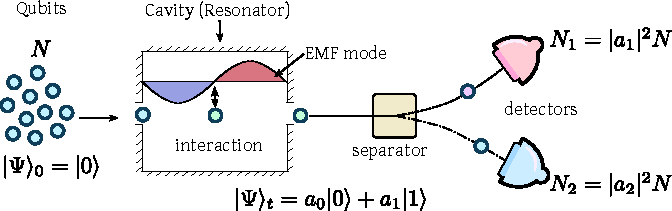
\includegraphics[scale=1.0]{qubitNumberOperatorMeaning}
	\caption{Qubits initially in the ground state $\ket{0}$ travel through a cavity resonator with an electromagnetic field mode attuned to the qubits transition energy $\Delta E=\hbar\omega$. After interaction, the state of each qubit changes to $\ket{\Psi_t}$. Then the qubits are "measured"/separated into two groups, based on their final state.}
	\label{fig:qubitNumberOperatorMeaning}
\end{figure}

Next, consider an experiment schematically shown in Figure \ref{fig:qubitNumberOperatorMeaning}. In this experiment a large number $N$ of qubits start in the ground state $\ket{0}$ and go through a region (cavity) where they can interact with an oscillating electromagnetic field (mode). After leaving the cavity, each qubit goes through a special device which splits the beam into two parts, depending on the measured state of a qubit. The top detector detects $N_1$ qubits in state $\ket{1}$, the bottom detector detects $N_2$ qubits in ground state. The $N_1$  qubits correspond to the number of energy quanta absorbed from cavity. This number can be expressed as
\[
N_1=N |a_1|^2=N\bra{\Psi_t}\op{n}\ket{\Psi_t}\,.
\]  
In other words, the expectation value of the operator $\op{n}$ determines the number of energy quanta absorbed from the mode of electromagnetic field inside the cavity.
 

\section{Quantum Oscillator}\label{sec:QuantumOscillator}
The \emph{principle of the quantization of action} can be applied to harmonic oscillator. The result is the quantization of energy levels. 

The energy of a harmonic oscillator can be expressed in terms of the maximum momentum $p_m$ or in terms of the maximum displacement $x_m$:
\[
H = \frac{p_m^2}{2m}\quad\textrm{ or }\quad H=\frac{kx_m^2}{2}\,.
\]
Multiplying these two equalities and recalling that $\omega^2=k/m$, we obtain
\[
H = \frac{\omega x_m p_m}{2}\,.
\]
The path which the state vector $\ket{\xi}=(x,p)$ follows in phase space is an ellipsis with the major semi-axes $x_m$ and $p_m$. The area of this ellipsis is $A=\pi x_m p_m$. Therefore, the connection between the energy of harmonic oscillator and the area is given by
\[
H=\frac{\omega}{2\pi}A\,.
\]
The area $A$ is a physical quantity with the units of action.

As shown in Figure \ref{fig:phaseSpaceQuantum}(a), areas in phase space have the smallest size limited by the elementary quantum of action $h$ -- known as Planck constant. The quantization of action and, consequently, the quantization of phase-space area, has two important implications for harmic oscillator.
\begin{figure}[htbp]
	\centering
	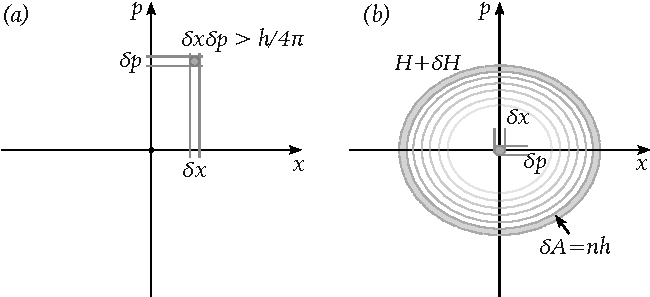
\includegraphics[scale=1.0]{phaseSpaceQuantum}
	\caption{Areas of phase-space regions have the units of action. Quantization of action implies quantization of phase-space area. (a) The smallest area in phase space is limited by the fundamental quantum of action $h$ -- Planck's constant. (b) Area of the ellipsis inside the path of harmonic oscillator is proportional to its energy. Quantization of area leads to the quantization of energy of harmonic oscillator.}
	\label{fig:phaseSpaceQuantum}
\end{figure}

First, every time an oscillator absorbs some energy $\Delta E$, the maximum deviation and the maximum momentum increase. The ellipsis in phase space increases its area. But since the area in phase space can't grow continiously--changes in discrete quanta $\delta A=h$--we must have discreete changes in energy. Second, the existence of the elementary quantum of action and the smallest are in phase space, require that the lowest energy state of harmonic oscillator is described not by a point in phase space, but by an elementary ellipsis such that $A_0=\delta x\delta p\propto h$. Putting these two ideas together, we conclude that the area of the ellipsis can be written as
\[
A_n = A_0 + nh\,.
\]
The energy of the oscillator then takes the form
\[
H=n\hbar\omega + E_0\,,
\]
where $\hbar=h/2\pi$ is called \emph{reduced Planck's constant}, and $E_0$ is the lowest energy of the harmonic oscillator. From the expression for $H$ follows that harmonic oscillator can be in a countable set of states, growing in energy from $E_0$ by a fixed step $\hbar\omega$. 

The energy of the lowest state can be written in terms of the step size $\hbar\omega$: $E_0=e_0\hbar\omega$, where $e_0$ is some number (it will be found later). Finally, we can write the energy of harmonic oscillator as follows:
\[
H=\hbar\omega(n + e_0)\,.
\]

\subsection{Hamiltonian Operator}
For any quantum system with descrete energy states $E_0, E_1, E_2,\ldots, E_n\ldots$ the Hamiltonian operator can be written in terms of projectors:
\[
\op{H}=\int E_k\ketbra{k}{k}\,,\quad k=0,1,2,\ldots,n\ldots 
\]
For harmonic oscillator $E_k=E_0+k\hbar\omega$ for $n>1$ and the Hamiltonian operator can be written as follows
\[
\op{H} = \int (E_0+k\hbar\omega)\ketbra{k}{k}\,.
\]
The number $k$ tells how many excitations quantum oscillator absorbed to reach the energy state $\ket{k}$.
Opening the parentheses and recalling that
\[
\int\ketbra{k}{k}=\op{I}\,,
\] 
we obtain 
\[
\op{H} = E_0\op{I}+\hbar\omega \int k\ketbra{k}{k}\,.
\]
This expression is very similar to the Hamiltonian of a qubit 
\[
\op{H}_{qb}=E_g\op{I}+\hbar\omega\op{n}
\]
where $\op{n}=\op{\sigma_\plus}\op{\sigma_\minus}$ is a number operator. The similarity is not accidental, as the operator $\op{n}=\int k\ketbra{k}{k}$ plays the role of the number operator. Indeed, it is easy to check by direction application that:
\[
\op{n}\,\ket{n}=n\ket{n}\,.
\]
In other words, the energy states $\ket{n}$ of harmonic oscillator, are the eigen-states of the number operator $\op{n}$ with the eigen-value $n$ corresponding to the number of excitation level.
\begin{exercise}
	Prove that $\op{n}\,\ket{n}=n\ket{n}$ by direction application of the operator $\op{n}=\int k\ketbra{k}{k}$.
\end{exercise}

The expression for the number operator $\op{n}$ can be obtained in a different way. First note that
\[
\op{H}\,\ket{n}=E_n\ket{n}\,,\quad\textrm{ where } E_n = E_0 + n\hbar\omega\,.
\]
From this follows
\[
(\op{H}-E_0\op{I})\,\ket{n}=n\hbar\omega\,\ket{n}\,,
\]
and, consequently, 
\[
\frac{(\op{H}-E_0\op{I})}{\hbar\omega}\,\ket{n}=n\,\ket{n}\,.
\]
The operator on the left hand side of this equation is the number operator $\op{n}$. It can be simplified once we recall that
\[
\op{H}=\int E_k\ketbra{k}{k}\quad\textrm{ and }\quad \op{I}=\int\ketbra{k}{k}\,.
\]
Using these relations, we first write
\[
\op{H}-E_0\op{I}=\int (E_k-E_0)\ketbra{k}{k}\,.
\]
Then, remembering that $E_k=E_0+k\hbar\omega$, we immediately arrive at
\[
\op{n}=\frac{(\op{H}-E_0\op{I})}{\hbar\omega}=\int k\ketbra{k}{k}\,.
\]
Thus, the operator of quantum harmonic oscillator can be written in the following form:
\[
\op{H}_{osc}=E_0\op{I}+\hbar\omega\op{n}\,.
\]
\subsection{Ladder Operators}
The number operator for qubit could be expressed as the product of two simple operators that raised or lowered qubit states:
\[
\op{n} = \op{\sigma}_\plus\op{\sigma}_\minus\,.
\]
The idea of raising and lowering states is also applicable to harmonic oscillator. Similar to qubit, we can write such operators as tensor products:
\[
\op{a}_\plus = \ketbra{n+1}{n}\textrm{ and }\quad\op{a}_\minus=\ketbra{n-1}{n}\,.
\]
Unfortunately, these operators will act properly only on the state $\ket{n}$.
\begin{exercise}
	Evaluate (a) $\op{a}_\plus \,\ket{n}$; (b) $\op{a}_\minus \,\ket{n}$; (c) $\op{a}_\plus \,\ket{n+m}$; (d) $\op{a}_\plus \,\ket{n+m}$.
\end{exercise}
It is easy to fix this problem by summing over all states:
\[
\op{a}_\plus=\int \ketbra{k+1}{k}\quad\textrm{ and }\quad \op{a}_\minus=\ketbra{0}{0}+\int \ketbra{m-1}{m}\,,\quad m > 0\,.
\]
The first term in the expression for $\op{a}_\minus$ ensures that the vacuum state remains unchanged: $\op{a}_\minus\,\ket{0}=\ket{0}$.
\begin{exercise}
	Evaluate (a) $\op{a}_\plus \,\ket{n}$; (b) $\op{a}_\minus \,\ket{n}$.
\end{exercise}
Let's check whether $\op{a}_\plus\op{a}_\minus$ yields the number operator $\op{n}=\int k\ketbra{k}{k}$. Even without explicitely evaluating the composition $\op{a}_\plus\op{a}_\minus$ we can see that it is unlikely to contain the required factor $k$.
\begin{exercise}
	Show that $\op{a}_\plus\op{a}_\minus=\ketbra{1}{0}-\ketbra{0}{0}+\op{I}$.
\end{exercise}

To find better operators for raising and lowering states of harmonic oscillator, we can taken a closer look at the qubit case. There we had $\op{\sigma}_\plus\,\ket{0}=1\ket{1}$ and $\op{\sigma}_\minus\,\ket{1}=1\ket{0}$\,. We explicitely added "1" in front of the final states, to highlight the following property of the $\op{\sigma}$-operators:
\[
\op{\sigma}_\plus\,\ket{k}=\sqrt{k+1}\ket{k+1}\quad\textrm{ and } \op{\sigma}_\minus\,\ket{k}=\sqrt{k}\ket{k-1}\,.
\]
Thus, we can "upgrade" the raising and lowering operators $\op{a}_\plus$ and $\op{a}_\minus$ to include the information about the state they act on. We want them to behave as follows:
\[
\op{a}_\plus\,\ket{k}=\sqrt{k+1}\ket{k}\quad\textrm{ and }\quad \op{a}_\minus\,\ket{m}=\sqrt{m}\ket{m-1}\,.
\]
\begin{exercise}
	Evaluate $\left(\op{a}_\plus\right)^p\,\ket{0}$.
\end{exercise}
\begin{exercise}
	(a) Show that the upgraded operators have the property 
	\[
	\op{a}_\plus\op{a}_\minus\,\ket{m}=m\ket{m}\quad m>0\,.
	\]	
	(b) Evalulate $\op{a}_\minus\op{a}_\plus\,\ket{m}$.
\end{exercise}
\begin{exercise}
	(a) Show that 
	\[
	\op{a}_\minus\op{a}_\plus-\op{a}_\plus\op{a}_\minus=\op{I}\,.
	\]	
\end{exercise}

Such raising and lowering operators (also called \emph{ladder operators}) are very useful when working with quantum harmonic oscillators. In terms of the ladder operators, the Hamiltonian of quantum oscillator is written as
\[
\op{H}_{osc} = \hbar\omega\op{n}+E_0\op{I}\,,
\]
where the number operator $\op{n}=\op{a}_\plus\op{a}_\minus$. 


\subsection{Conjugation}
The raising operator $\op{a}_\plus$ can be written in terms of the tensor products:
\[
\op{a}_\plus=\int_0 \sqrt{k+1}\ketbra{k+1}{k}\,.
\]
If we limit the lowering operator to states $\ket{m}$ with $m>0$, then it also allows a simple representation
\[
\op{a}_\minus=\int_1 \sqrt{m}\ketbra{m-1}{m}\,.
\]
By changing the summation variable $m-1=k$ (and, therefore, $m=k+1$), we can re-write the summation over $k=0,1,2\ldots$:
\[
\op{a}_\minus=\int_0 \sqrt{k+1}\ketbra{k}{k+1}\,.
\]
Now the expression for $\op{a}_\minus$ became similar to the expression for $\op{a}_\plus$, with the exception that the order of states in the tensor product is flipped:
\[
\ketbra{k+1}{k}\leftrightarrow \ketbra{k}{k+1}\,.
\]
This change of order of factors in a tensor product is called \emph{conjugation}. The operators $\op{a}_\minus$ and $\op{a}_\plus$ are therefore related to each other via the \emph{conjugation operation}. These operators are said to be \emph{conjugates} of each other. 

The relation of conjugation gives some insight into what the lowering operator $\op{a}_\minus$ does to the vacuum state:
\[
\op{a}_\minus\,\ket{0}=\int_0  \sqrt{k+1}\ket{k}\braket{k+1}{0}=0\int_0\sqrt{k+1}\ket{k}=0\ket{\infty}\,,
\]
where we introduced a vector 
\[
\ket{\infty}=\ket{0}+\sqrt{2}\ket{1}+\sqrt{3}\ket{2}+\ldots+\sqrt{n+1}\ket{n}+\ldots
\]
Obviously, $\ket{\infty}\ne\ket{0}$. The overall factor of zero negates any possible contributions of $\ket{\infty}$, making the product $0\ket{\infty}$ a special "zero vector" $\ket{z_0}$, with the natural property
\[
\ket{k}+\ket{z_0}=\ket{k}\,.
\]
The vector $\ket{z_0}$ does not correspond to any physical state, but represents a mathematical "zero vector". Since for all mathematical manipulations the vectors $0\ket{\infty}$ and $0\ket{0}$ are equivalent,
we can express the action of the lowering operator $\op{a}_\minus$ on the vacuum state as follows:
\[
\op{a}_\minus\,\ket{0}=0\ket{0}\,.
\]
Finally, the action of the number operator $\op{n}=\op{a}_\plus\op{a}_\minus$ on the vacuum state can be evaluated:
\[
\op{a}_\plus\op{a}_\minus\,\ket{0}=\op{a}_\plus(\op{a}_\minus\,\ket{0})=0(\op{a}_\plus\,\ket{0})=0\ket{1}=0\ket{0}\,,
\]
here we used the mathematical equivalence of states $0\ket{1}$ and $0\ket{0}$.

\begin{mybio}{Dagger Notation}
	The relation of conjugation between operators is denoted using a special notation. For example, if we denote the lowering operator $\op{a}_\minus$ simply as $\op{a}$, then its conjugate operator-- raising operator-- is denoted using a special "dagger" symbol as the superscript:
	\[
	\op{a}_\plus = \op{a}^\dagger\,.
	\]
	The use of dagger notation is standard in quantum theory. 
	
	Let's use the dagger notation to summarize the basis facts about the ladder operators, the number operator, and the Hamiltonian of quantum oscillator.
	First, raising and lowering properties:
	\[
	\op{a}\,\ket{n}=\sqrt{n}\ket{n-1}\,,\qquad\op{a}^\dagger\,\ket{n}=\sqrt{n+1}\ket{n+1}\,.
	\]
	Second, number operator and commutator:
	\[
	\op{a}^\dagger\,\op{a}\,\ket{n}=n\ket{n}\,,\qquad \op{a}\,\op{a}^\dagger-\op{a}^\dagger\,\op{a}=\op{I}\,.
	\]
	Finally, conjugation relation between the ladder operators:
	\[
	\op{a}\overset{\dagger}{\longrightarrow}\op{a}^\dagger\,.
	\]
\end{mybio}
\subsection*{Normal Order}
\begin{exercise}
	Ladder operators are used many important applications of quantum theory. Often one encounters expressions with several operators in no particular order, for example $\op{X}=\op{a}^\dagger\,\op{a}^2\,\op{a}^\dagger\,\op{a}$. For calculations it is necessary to rearrange these operators into a \emph{normal order} where all raising operators appear on the left, before the lowering operators.
	
	Use the commutation relation $\op{a}\,\op{a}^\dagger-\op{a}^\dagger\,\op{a}=\op{I}$ to put $\op{X}$ into a normal order.
\end{exercise}


\subsection{Canonical Commutation}
The Hamiltonian operator for quantum harmonic oscillator can be written in different ways. One way relies on energy eigen-values $E_k$:
\[
\op{H}=\int_0 E_k\ketbra{k}{k}\,.
\]
Another way utilizes raising and lowering operators:
\[
\op{H}=\hbar\omega \op{a}^\dagger\,\op{a}+E_0\op{I}\,.
\]
However, the starting point was the expression in terms of position and momentum. The question then becomes whether we can introduce \emph{position and momentum operators} such that for harmonic oscillator we get
\[
\op{H}=\frac{\op{p}^2}{2m}+\frac{m\omega^2\op{x}^2}{2}\,.
\]
We already saw in Exercise X the hint that some relationship must exist between the operators $\op{a}$, $\op{a}^\dagger$ and $\op{x}$, $\op{p}$. Such relationship must be linear in order to transform the expression for $\op{H}$ quadratic in terms of raising and lowering operator
\[
\op{H}=E_0\op{a}\,\op{a}^\dagger+(\hbar\omega-E_0)\op{a}^\dagger\,\op{a}=\square\,\op{a}\,\op{a}^\dagger+\square\, \op{a}^\dagger\,\op{a}
\]
into the expression quadratic in terms of position and momentum
\[
\op{H}=\square\, \op{p}^2+\square\, \op{x}^2\,.
\]
We are thus looking for a linear transformation
\[
\op{x} = A\,\op{a}+B\,\op{a}^\dagger\quad\textrm{ and }\quad \op{p}=C\,\op{a}+D\,\op{a}^\dagger
\]
which will lead to the Hamiltonian operator $\op{H}=E_0\op{a}\,\op{a}^\dagger+(\hbar\omega-E_0)\op{a}^\dagger\,\op{a}$.
\begin{exercise}
	Show that the Hamiltonian operator for harmonic oscillator in terms of the unknown coefficients $A, B, C$ and $D$ has the form:
	\begin{align*}
	\op{H}= & \left(\frac{C^2}{2m}+\frac{m\omega^2A^2}{2}\right)\op{a}^2+\left(\frac{D^2}{2m}+\frac{m\omega^2B^2}{2}\right)\op{a}^\dagger+\\
	+& \left(\frac{CD}{2m}+\frac{m\omega^2 AB}{2} \right)\op{a}\,\op{a}^\dagger+\left(\frac{CD}{2m}+\frac{m\omega^2 AB}{2} \right)\op{a}^\dagger\,\op{a}\,.
\end{align*}
\end{exercise}
\begin{exercise}
	Using the result of the previous exercise, show that it implies that $E_0=\hbar\omega/2$.
\end{exercise}
\begin{exercise}
	Using the results of the two previous exercises, show that the four unknown coefficients $A, B, C$ and $D$ satisfy the following equations:
	\[
	C^2=-(m\omega A)^2\,,
	\]
	\[
	D^2=-(m\omega B)^2\,,
	\]
	and
	\[
	CD+(m\omega)^2AB=m\hbar\omega\,.
	\]
\end{exercise}
\begin{exercise}
	Using the result of the previous exercise, show that $CD=(m\omega)^2AB$ (convince yourself that $CD$ can't be $CD=-(m\omega)^2AB$!). Then show that one possible solution is the set of coefficients:
	\[
	A=B=\sqrt{\frac{\hbar}{2m\omega}}\,,
	\]
	and
	\[
	C=-D=-\op{J}\sqrt{\frac{\hbar m\omega}{2}}\,.
	\]
\end{exercise}

With the steps outlined above, we obtain the following expressions for the operators of position and momentum:
\[
\op{x}=\sqrt{\frac{\hbar}{2m\omega}}\left(\op{a}^\dagger+\op{a}\right)=x_\omega\left(\op{a}^\dagger+\op{a}\right)
\]
and
\[
\op{p}=\op{J}\sqrt{\frac{\hbar m\omega}{2}}\left(\op{a}^\dagger-\op{a}\right)=\op{J} p_\omega\left(\op{a}^\dagger-\op{a}\right)\,.
\]
Using these relations, it is now easy to find so called \emph{canonical commutation relation} for the basic physical operators of position and momentum. First, we find
\[
\op{x}\op{p}=\op{J}\frac{\hbar}{2}\left(\op{a}^\dagger\op{a}^\dagger-\op{a}\op{a}+\op{a}\op{a}^\dagger-\op{a}^\dagger\op{a}\right),
\]
then
\[
\op{p}\op{x}=\op{J}\frac{\hbar}{2}\left(\op{a}^\dagger\op{a}^\dagger-\op{a}\op{a}+\op{a}^\dagger\op{a}-\op{a}\op{a}^\dagger\right).
\]
Subtracting the latter equation from the former, we arrive at
\[
\op{x}\op{p}-\op{p}\op{x}=\lbrack \op{x},\op{p}\rbrack=\op{J}\hbar\lbrack \op{a},\op{a}^\dagger\rbrack=\op{J}\hbar\,.
\]

\section{Physical Realization of Qubits}
Recall that harmonic oscillator is \emph{any} physical system with the Hamiltonian in the form
\[
H = \frac{p^2}{2m}+\frac{kx^2}{2}\,.
\] 
Many physical systems can be described using this Hamiltonian and thus provide specific \emph{realizations} of 
the oscillator model. Similarly, many concrete physical systems realize the idea of a qubit.

\section{Interacting Qubits}\label{sec:InteractingQubits}
Isolated quantum systems are idealizations. Interactions between systems are not only hard to  avoid, but are often desirable for practical purposes. We now turn our attention to the interaction between a pair of simplest quantum systems -- quantum qubits.

\subsection{Joint State}
Treating a pair of qubits as a single quantum system implies describing the state of two qubits with a single state vector $\ket{\Psi}$.  It is called a \emph{joint state} vector and is used to describe the results of  measurements performed on a pair of qubits.

To measure two separate parts of a single quantum system one may use two detectors. Each detector measures a single qubit and finds it in either state $\ket{0}$ or $\ket{1}$ with different probabilities. The results of a \emph{joint measurement} can be expressed as a linear combination of all possibilities:
\[
\ket{\Psi} = c_{00}\ket{0}\ket{0} + c_{01}\ket{0}\ket{1}+c_{10}\ket{1}\ket{0}+c_{11}\ket{1}\ket{1}\,.
\]
For example, if all results are equally probable, the state of the qubit-pair system can be written as follows:
\[
\ket{\Psi_0} = \left(\ket{0}\ket{0} + \ket{0}\ket{1}+\ket{1}\ket{0}+\ket{1}\ket{1}\right )/2\,.
\]
There are no \emph{correlations} between the measurements for this state. Two qubits are not only spatially separated, but also \emph{statistically unrelated}. In this case each qubit can be assigned its own state vector and the joint state $\ket{\Psi}$ is a product of two states:
\[
\ket{\Psi_0}=\ket{\psi}\ket{\phi}
\]
where $\ket{\psi}=\left(\ket{0}+\ket{1}\right)/\sqrt{2}$ and $\ket{\phi}=\left(\ket{0}+\ket{1}\right)/\sqrt{2}$.

Whenever the results from two detectors are correlated, the separation of a qubit pair into independent parts becomes impossible. The state $\ket{\Psi}$ then can't be factorized: $\ket{\Psi}\ne \ket{\psi}\ket{\phi}$. Indeed, suppose the state is 
\[
\ket{\Psi_1} = \left(\ket{0}\ket{0} + \ket{1}\ket{1}\right )/\sqrt{2}\,.
\]
Assuming that $\ket{\Psi}=\ket{\psi}\ket{\phi}$ and $\ket{\psi}=a\ket{0}+b\ket{1}$ and $\ket{\phi}=c\ket{0}+d\ket{1}$, we get four requirements for the coefficients $a,\,b,\, c$ and $d$:
\begin{align*}
	ac & = 1/\sqrt{2}\,, & ad=0\\
	bd & = 1/\sqrt{2}\,, & bc=0\,.
\end{align*}
These requirements can't be satisfied, because $a$ and $d$ can't be zero, while their product must be zero (similarly $b$ and $c$). 

The state $\ket{\Psi_1} = \left(\ket{0}\ket{0} + \ket{1}\ket{1}\right )/\sqrt{2}$ is an example of \emph{entangled} state of a qubit pair. It illustrates a peculiar quantum situation when the complete knowledge about the joint system does not mean complete knowledge of its "parts". In other words, in a strongly \emph{correlated system} there are no independent parts which can be described with their own individual state vectors. Qubit pair acts as \emph{one inseparable whole}.

\begin{exercise}
	Suppose a qubit pair is in the state 
	\[
	\ket{\Psi_2} = \left(\ket{0}\ket{1} + \ket{1}\ket{0}\right )/\sqrt{2}\,.
	\]
	Show that this state can't be written as the product state:
	\[
	\ket{\Psi_2} \ne \ket{\psi}\ket{\phi}\,.
	\]
\end{exercise}



\subsection{Creating Entanglement}
How do qubits become \emph{entangled}? Let's show that an interaction between qubits, responsible for the transfer of energy from the first qubit to the second, can, in certain scenarios, lead to an entangled state. The mechanism described below is universal in the sense that it works for any two interacting quantum systems, not just a pair of qubits.

Energy exchange between two qubits implies the following transition:
\[
\ket{1}\ket{0}\quad\longrightarrow\quad\ket{0}\ket{1}\,.
\]
This is a process in which the first qubit is initially excited, and the second qubit is in the ground state, but in the end the first qubit drops into the ground state, while the second qubit becomes excited. Mathematically, this transition is described by a product of operators:
\[
\op{T}_1 = \op{\sigma}_1\otimes \op{\sigma}^\plus_2 = \op{\sigma}_1\op{\sigma}^\plus_2\,.
\]

Interaction leading to an energy exchange between two qubits can be 

\[
\op{H}=\op{H}_1\op{I}_2+\op{I}_1\op{H}_2+\epsilon\left(\op{\sigma}_1\op{\sigma}^\plus_2+\op{\sigma}^\plus_1\op{\sigma}_2\right)\,.
\]

\begin{mybio}{Where is Energy?}
	When a qubit pair is entangled, neither qubit has definite energy. However, the system as a whole does have a certain energy. How is this energy "divided" between the qubits?
\end{mybio}


\subsection{Computational Basis}
The four joint states of a qubit pair
\[
\ket{\Upsilon}_1 = \ket{0}\ket{0},\,\,\ket{\Upsilon}_2 = \ket{0}\ket{1},\,\,
\ket{\Upsilon}_3 = \ket{1}\ket{0},\,\,\ket{\Upsilon}_4 = \ket{1}\ket{1}\
\]
are called \emph{computational basis}.


Q: Are there other states, which are also basis and product? Smth like
\[
\ket{\Xi}=\ket{+}\ket{+}\,.
\]

\subsection{Bell States}
\[
\ket{\Phi}^{+}\,,\quad\ket{\Phi}^{-}\,,\quad
\ket{\Psi}^{+}\,,\quad\ket{\Psi}^{-}\,.
\]


\subsection{GHZ State}\label{sec:GHZState}
We are looking for a binary operator $\op{\sigma}$ that yields a number
based on two vectors:
\[
\ketbra{\sigma}{\sigma}\,\vec{a}\,\vec{b}=x\,.
\]


\section{Quantum Field}\label{sec:QuantumField}
We are looking for a binary operator $\op{\sigma}$ that yields a number
based on two vectors:
\[
\ketbra{\sigma}{\sigma}\,\vec{a}\,\vec{b}=x\,.
\]

We are looking for a binary operator $\op{\sigma}$ that yields a number
based on two vectors:
\[
\op{\sigma}\,\vec{a}\,\vec{b}=x\,.
\]
We will call this operator $\op{\sigma}$ \emph{dol}-operator\footnote{This is not a
standard terminology. }, based on the key letters of the phrase
``\underline{d}egree of \underline{o}ver\underline{l}ap''.

\begin{myrem}{Reminder}
When we say that an operator $\op{\Gamma}$ is given or known, we
mean that we know how it acts on \emph{any vector} $\vec{a}$:
\[
\op{\Gamma}\,\vec{a} = x_a\,.
\]
\end{myrem}

Array of equations:
\begin{eqnarray}
  \op{\Gamma}_1\,\vec{e}_1 & = & 1\,\\
  \op{\Gamma}_1\,\vec{e}_2 & = & 0\,\\
  \op{\Gamma}_1\,\vec{e}_3 & = & 0\,\\
  \ldots
\end{eqnarray}

\subsection{Quantum States of Light}

\section*{Chapter Highlights}
{\setstretch{1.5}\chhc
  \it
\begin{itemize}
\item Two vectors can be compared for similarity by calculating the
  ``degree of overlap''. The longer two vectors are and the closer
  their mutual direction -- the greater the overlap is.
\item Degree of overlap can be described by a binary linear operator
  $\op{\sigma}$. This operator is closely related to the concept of
  scalar product of two vectors.
\item When scalar product (or, equivalently, degree of overlap) is
  defined for vectors, each vector receives a ``special relative'' --
  conjugate vector -- that lives in different vector space, called
  conjugate or dual space.
\item When the degree-of-overlap operator $\op{\sigma}$ is partially
  applied, the result is a unary linear operator that yields a number
  for every input vector. Importantly, such an operator is also a
  vector, albeit not an arrow-like vector.
\end{itemize}

}


%\chapterimage{chapterImageDefault.pdf}
%\chapterimage{relativity.pdf}
%\input{../06Appendices/appendices.tex}


%----------------------------------------------------------------------------------------
%	PART
%----------------------------------------------------------------------------------------

%% \part{Waves and Fields}

%\part{Appendix}
\chapterimage{pics/chapterImageApplications.pdf}
%\chapterimage{relativity.pdf}
\graphicspath{{../06Applications/pics/}}

\chapter{Applications}\label{ch:Applications}
\lettrine[lines=2]{\color{darkocre}W}{e} are now ready to appreciate
how tensors are used in ``real life''. In this chapter we will
encounter examples of
tensors that are used in mathematics, physics, and engineering. 

\begin{myprereq}{Prerequisite Knowledge}
	To fully understand the material of this chapter, readers should be comfortable with the following concepts:
	
	\begin{itemize}
		\item \phantom{phantom}
		\vspace{-0.5cm}
		\item State
		\item Dynamical equations
	\end{itemize}	
\end{myprereq}

\section{Hydrogen-like Atoms}
We will start with the simplest atomic system: Hydrogen atom.

\subsection{Hydrogen Atom}
The most abundant element in the observable universe is hydrogen. A
hydrogen atom has two components: heavy nucleus (proton) and light
``shell'' (electron). The two components can be separated in the
process of \emph{ionization}. A significant energy is required to
tear-off the shell:
\[
E_{ion} = 2.18\times 10^{-18} (J) = 13.6\, (eV)\,.
\]
These numbers do not look big; however, they correspond to an extremely
high temperature:
\[
T_{ion} = \frac{E_{ion}}{k} = \frac{2.18\times 10^{-18}}{1.38\times
	10^{-23}} = 157\,887\, (K)\,.
\]
This is almost 30 times higher than the temperature near the
``surface'' of the sun; the estimated temperature in the core of the
sun is about 100 times higher than the hydrogen ionization
temperature.

The bottomline is that in normal conditions the electron is reliably
\emph{trapped/localized/confined} in a small region near the nucleus. The
diameter of hydrogen atom provides a convenient ``scale'' for
distances in atomic world:
\[
d_H \approx 1\, \r{A}\,\qquad \r{A}\textrm{ngstrom } = 10^{-10}\, (m)\,.
\]

\begin{tcolorbox}[colback=white!85!ocre, title=$\circledast\,$Illustration]
	If every person on earth had a hydrogen atom and placed it in a single
	row next to each other, then the resulting chain would be about a
	meter long.
\end{tcolorbox}

\begin{tcolorbox}[colback=white!85!ocre, title=\r{A}ngstrom]
	Angstrom is a convenient unit for measuring distances between atoms
	inside solid bodies. For example, copper atoms are about 2.8 \r{A} in
	diameter and are arranged in a crystal with the distance between the
	nearest neighbors $d\approx 3.6$ \r{A}.
\end{tcolorbox}

To see how those values for the ionization energy and atomic radius
appear, let us consider the following model of the atom, shown in the
Figure \ref{fig:hydrogenAtom}.
\begin{figure}[htbp]
	\centering
	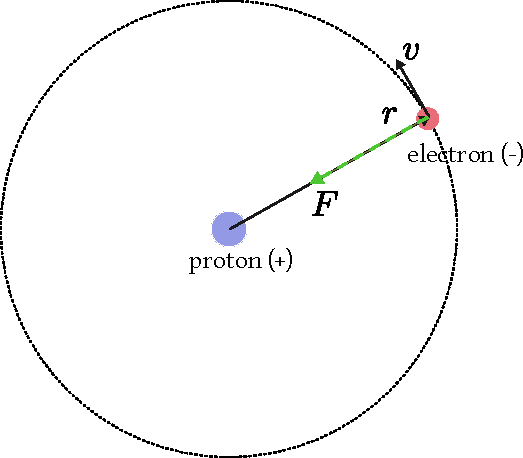
\includegraphics[scale=0.6]{hydrogenAtom}
	\caption{Planetary model of hydrogen atom.}
	\label{fig:hydrogenAtom}
\end{figure}

The circular motion of the electron around the nucleus is
mathematically similar to the problem of a planet circling a
star. Using the second law of Newton and the expression for the
Coulomb's force, we can write
\[
\frac{m_ev^2}{r} = k\frac{q_e^2}{r^2}\,,
\]
where
\[
k = \frac{1}{4\pi\varepsilon_0}\,.
\]

Newtonian momentum is given by $p=mv$; from the motion equation
above, we find
\[
p^2 = k\frac{m_e q_e^2}{r}\,.
\]

\begin{figure}[htbp]
	\centering
	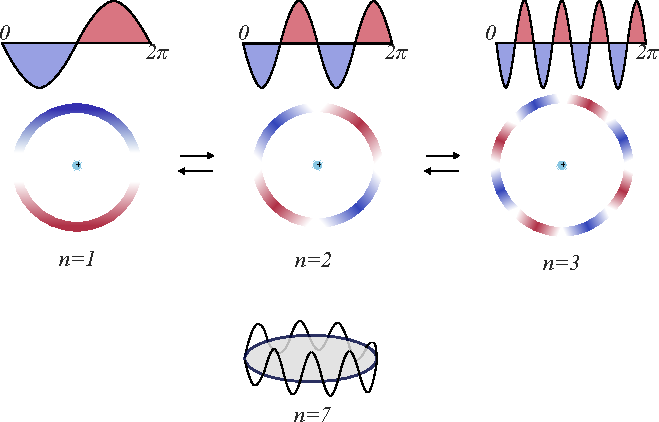
\includegraphics[scale=1.0]{hydrogenAtomOrbits}
	\caption{Orbits allowed by the semi-quantum model.}
	\label{fig:hydrogenAtomOrbits}
\end{figure}

Using de Broglie hypothesis about the relation between momentum and
wavelength
\[
p\lambda = h\,,
\]
and combining it with \emph{quantization hypothesis}:
\[
n\lambda = 2\pi r
\]
or, equivalently,
\[
pr = n\frac{h}{2\pi} = n\hbar\,
\]
we find possible solutions for the radius of the ``orbit'':
\[
r_n = \frac{\hbar^2 n^2}{km_e q_e^2}\qquad n = 1, 2, 3,\ldots
\]
The smallest value of the radius is
\[
a_0 = r_1 = \frac{4\pi\varepsilon_0 \hbar^2}{m_e q_e^2} = 0.523\,\r{A}\,.
\]
It is called \emph{Bohr radius}. Thus, the smallest diameter of
electron's orbit is about 1 \r{A}ngstrom.
\begin{exercise}
	Find the numbers for which the radius of electron ``orbit'' equals:
	1) 1 mm; 2) 1 cm; 3) 1 m.
\end{exercise}

How fast does the electron move around the nucleus? The velocity
of the electron is
\[
v = \sqrt{\frac{kq_e^2}{m_e r}}\,.
\]
Substituting $r_n = a_0 n^2$ we get
\[
v_n = \frac{1}{n}\sqrt{\frac{kq_e^2}{m_e a_0}} = \frac{v_1}{n}\,.
\]
The value of $v_1$ is
\[
v_1 = 2.19\times 10^6\,(m/s)
\]
Although this is a big number, it is much smaller than the speed of
light; we are therefore justified in using Newtonian mechanics and not
taking relativity into account.

\begin{tcolorbox}[colback=white!85!ocre, title=$\circledast\,$Fun Fact]
	The ``quantization'' of orbit radius can be found even for planets in
	solar system. If we denote the distance between the earth and the sun
	as $A$ (called \emph{astronomical unit}), then the distances to
	planets from the sun are given by the formula
	\[
	r_n = \frac{A}{10}(4+3\times 2^n)\,.
	\]
	This relation is known as \emph{Titius-Bode} law. It works remarkably
	well for all planets from Venus ($n=0$) to Uranus ($n=6$).
\end{tcolorbox}

How strong is the electron attracted to the nucleus? The Coulomb force
between the charges is
\[
F = \frac{kq_e^2}{r^2}\,.
\]
Substituting $r_n = a_0 n^2$ we get
\[
F_n = \frac{kq_e^2}{a_0^2 n^4} = \frac{F_1}{n^4}\,.
\]
The value of $F_1$ is
\[
F_1 = 8.24\times 10^{-8}\,(N)
\]
This is a tiny force on the human scale of forces.
\begin{tcolorbox}[colback=white!85!ocre, title=$\circledast\,$Fun Fact]
	Even a baby ant has enough force to tear a hydrogen atom apart with
	its bare hands!
\end{tcolorbox}
Although the force acting on the electron is small on a human scale,
the acceleration ($a=v^2/r$) it produces is very large (on the human
scale, compare to $g$). This is due to extreme lightness of the
electron:
\[
m_e = 9.1\times 10^{-31}\, (kg)\,.
\]

What is the total energy of the hydrogen atom? It can be found as
follows:
\[
E_n = \frac{m_ev_n^2}{2}-k\frac{q_e^2}{r_n} = -\frac{E_1}{n^2}\,,
\]
where
\[
E_1 = k\frac{q_e^2}{2m_e a_0}\,.
\]
The value of $E_1$ is
\[
E_1 = 2.18\times 10^{-18}\, (J)\,.
\]
In atomic world a special unit of energy is used. It is the energy of
electon accelerated by a voltage drop of 1 Volt:
\[
E_{ev} = 1\,(V)\times q_e = 1.6\times 10^{-19}\, (J)\,.
\]
Using this atomic unit, the hydrogen atom has energy
\[
E_1 = 13.6\, (eV)\,.
\]

\begin{exercise}
	What is the frequency of revolution of electron around the nucleus
	for an orbit number $n$?
\end{exercise}

\subsubsection{Atoms Can't Exist?}
The model described above leads to the conclusion that atoms must not
exist for long. According to the theory of classical electrodynamics,
a charge moving in a circle will emit electromagnetic
waves with the frequency of revolution. As the atom loses its energy,
the electron spirals ever closer to the nucleus. Taking classical
electrodynamics into account, the life-time of a hydrogen atoms should
be about nanosecond. This contradicts the observation of stability of
atoms.

Niels Bohr suggested that the ``orbits'' represent so called
\emph{stationary states}, where electrons can ``move'' without
radiating away electromagnetic waves. Radiation only happens when
electron \emph{transitions} between stationary levels, for example
between 2 and 4. The energy carried away by the light is related to
the frequency of the electromagnetic wave $\nu$ as follows:
\[
\Delta E = E_m - E_n = h\nu_{nm}\qquad m > n\,.
\]

%\begin{tcolorbox}[colback=white!85!ocre, title=Exercise]
\begin{exercise}
	How much energy is required to ``move'' electron from the``orbit''
	of 1 mm to 1 cm? From 1 cm to 1m?
\end{exercise}
%\end{tcolorbox}

\subsubsection{Line Spectra Explained}
Using the results obtained above, we can now describe the spectra of
light emitted or absorbed by hydrogen.

The stationary states are discrete, therefore there are discrete
energies of transition between a pair of levels. When atom absorbs
electromagnetic radiation, electron ``jumps up'' to higher energy
level and farther distance. In the reverse process, electron ``jumps
down'' from higher level to lower one, resulting in emission.

The wavelength of the radiation is
\[
\lambda = cT = \frac{c}{\nu} = \frac{ch}{E_m - E_n}\,.
\]
Plugging in the expression for the energy, we get
\begin{equation}
	\lambda = \frac{ch}{E_1}\frac{n^2m^2}{m^2-n^2} = 91.127(nm)\times\frac{n^2m^2}{m^2-n^2}\,.
	\label{eq:lambdaSeries}
\end{equation}

A special case of this formula was discovered in 1885 by a Swiss
mathematician Johan Balmer. Analyzing the visible lines in the spectra
of hydrogen, he found some regularity in the wavelengths. Balmer
expressed it as follows:
\[
\lambda = B\frac{m^2}{m^2-2^2}\,,
\]
where $m > 2$ and $B=364.51$ nm.
Looking at (\ref{eq:lambdaSeries}), we can see that it can be written
for $n=2$ as
\[
\lambda = 91.127(nm)\times \frac{4m^2}{m^2-2^2} = 364.51(nm)\times \frac{m^2}{m^2-2^2}\,.
\]

%\begin{tcolorbox}[colback=white!85!ocre, title=Exercise]
\begin{exercise}
	According to the the formula  (\ref{eq:lambdaSeries}), how many
	hydrogen lines will be in the visible part of the spectrum (from
	400nm to 700nm)?
\end{exercise}
%\end{tcolorbox}

\begin{mybio}{Three Body Problem}
	The problem of hydrogen atom involves \emph{three} physical entities
	interacting with each other: Proton, electron, and electromagnetic
	field. Electron does not interact directly with the proton, it does
	so via the electric field of the nucleus. This is important to keep
	in mind, especially if we want to understand the phenomenon of
	\emph{spontaneous emission}.
\end{mybio}
\subsubsection{Spontaneous Emission and Cavity QED}
According to Schrodinger equation, an hydrogen atom with electron in any
statioary state $\qs{\Psi_n}$ with energy $E_n$ will remain in this
state \emph{forever}. In reality, every atom will randomly transition
into a state with lower energy, all the way to the lowest energy
state, emitting radiation as the result. This is called \emph{spontaneous
	emission}.

To describe spontaneous emission, one must account for the fact that
atom is not truly isolated and electron and proton are not the only
quantum systems in picture. There is an electromagnetic field with its
many modes-oscillators.

Interaction of atom-like quantum systems (qubits, quantum dots, atoms)
with quantum states of electromagnetic field is the focus of an exctiting
area of research called \emph{Cavity Quantum Electrodynamics} or \emph{cavity QED}.
\begin{figure}[htbp]
	\centering
	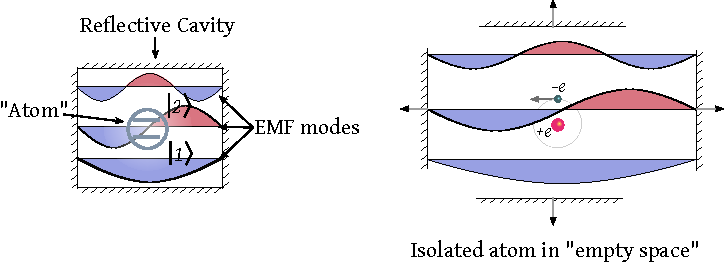
\includegraphics[scale=1.0]{cavityQED}
	\caption{Atom in ``empty space'' is a quantum system in a very large
		cavity, coupled to the modes-oscillators of electromagnetic field.}
	\label{fig:cavityQED}
\end{figure}

\subsection{Franck-Hertz Experiment}
The energy required for atoms to transition between different states may come not only from electromagnetic radiation ("photons"), but from kinetic energy of other particles bumping into atoms. Such a phenomenon was studied by James Franck and Gustav Hertz in 1914 using collisions of electrons with mercury atoms enclosed in a special vacuum tube\footnote{Interestingly, according to James Franck, neither he nor Gustav Hertz had any knowledge of Bohr's theory of atomic states when they performed their experiment.}. They showed that whenever electrons had a certain kinetic energy -- specific to mercury atoms -- they transfered this energy very efficiently (\emph{resonantly}) to mercury atoms. When the energies of electrons and mercury atoms were not matched, electrons scattered from the atoms \emph{elastically} -- without the loss of their kinetic energy.  The work of Franck and Hertz was recognized with 1925 Nobel Prize in Physics.

\subsubsection*{Idea}
The idea of Franck-Hertz experiment is illustrated in figure \ref{fig:franckHertzExperiment}. Its central part consists of a closed vacuum tube with mercury gas and several electric elements used as the source and sink of electrons.
\begin{figure}[htbp]
	\centering
	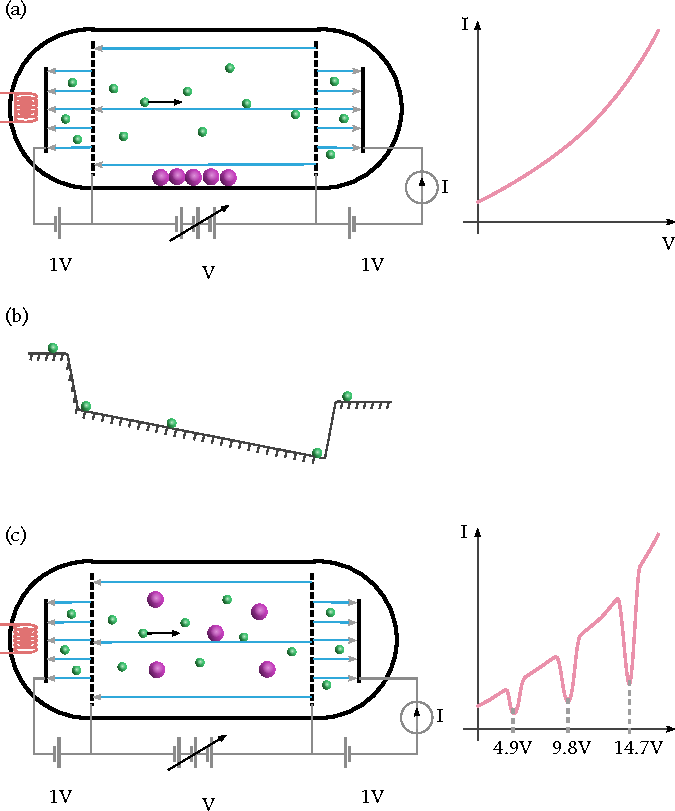
\includegraphics[scale=1.0]{franckHertzExperiment}
	\caption{(a) A vacuum tube is used to study the flow of electrons between two metal electrods under various conditions.; (b); (c).}
	\label{fig:franckHertzExperiment}
\end{figure}


\subsubsection*{Numbers}
At room temperature mercury is a liquid metal which can be easily evaporated by heating it up to 200$^\circ$C. It is thus not hard to create \emph{mercury gas}. The gas is \emph{monoatomic} -- consisting of single $Hg$ atoms, unlike molecular gases such as hydrogen $H_2$, oxigen $O_2$, or nitrogen $N_2$.

Each mercury atom contains 80 protons and 120 neutrons and is significantly heavier than an electron: $M_{Hg}\approx 4\times 10^5\,m_e$.  Consequently, an electron colliding with a mercury atom won't be able to impart any appreciable recoil speed or transfer energy to the latter. 
\begin{exercise}
	Show that for the head-on collision the speed of an initially stationary mercury atom after the collision becomes $v=2v_0\frac{m_e}{M_{Hg}}$.
\end{exercise}

\subsection{Stoke's Rule}
Stoke's rule.

\section{Rydberg Atoms}
When an atom has outer electron(s) excited into states with high excitation number  $n$, it is called a \emph{Rydberg atom}(CHECK!). Such atoms are of great importance for experiments of quantum physics.

\section{Quantum Dots}
Quantum dots can be viewed as \emph{artificial atoms} -- human-made physical structures designed to confine electrons in tiny volumes. As the result, quantum states of the trapped electrons form a discrete set not unlike the states of a hydrogen atom. \emph{Examples:???}

To illustrate the idea, consider an idealized case of an electron confined in one dimension in a region between $x=0$ and $x=L$.

\[
\ketbra{\alpha}{\beta}
\]
\[
E_n = -\frac{E_i}{n^2}\,.
\]

\section{Spontaneous Emission}
\[
\ketbra{\alpha}{\beta}
\]
\[
E_n = -\frac{E_i}{n^2}\,.
\]

\section{Stimulated Emission}
\[
\ketbra{\alpha}{\beta}
\]
\[
E_n = -\frac{E_i}{n^2}\,.
\]

\section{Lasers}
From the standpoint of quantum physics, lasers are special \emph{sources of excitation of electromagnetic field}. Laser's operation is based on the effect of {\bf L}ight {\bf A}mplification by the {\bf S}timulated {\bf E}mission of {\bf R}adiation (LASER).
\[
\ketbra{\alpha}{\beta}
\]
\[
E_n = -\frac{E_i}{n^2}\,.
\]



\section{Photoeffect}
\[
\ketbra{\alpha}{\beta}
\]
\[
E_n = -\frac{E_i}{n^2}\,.
\]

\section{Black Body Radiation}
\[
\rho_\nu = \frac{2h\nu^3}{c^2}\frac{1}{e^{h\nu/kT}-1}\,.
\]
\[
E_n = -\frac{E_i}{n^2}\,.
\]

\section{Conductors}
\[
\ketbra{\alpha}{\beta}
\]
\[
E_n = -\frac{E_i}{n^2}\,.
\]

\subsection{Heat Capacity}
Einstein's model.

\section{Entanglement}
Entanglement can be viewed as a physical resource of purely quantum nature. As a resource, entanglement facilitates several important processes related to processing of information.
\[
\ketbra{\alpha}{\beta}
\]
\[
E_n = -\frac{E_i}{n^2}\,.
\]

\subsubsection*{$\delta$-Notation}\index{Notation!delta}
When a quantity $x$ changes by a tiny amount, we will denote the
change using small Greek letter $\delta$ (delta) as follows:
\[
\colorboxed{red}{\delta x\textrm{ - tiny change of } x.}
\]
A convenient way to write all components of a second rank tensor is to
use table-like structure called \emph{matrix}\index{Matrix}:
\[
F^{\mu\nu}=
\begin{pmatrix}
  F^{00} & F^{01} & F^{02} & F^{03}\\
  F^{10} & F^{11} & F^{12} & F^{13}\\
  F^{20} & F^{21} & F^{22} & F^{23}\\
  F^{30} & F^{31} & F^{32} & F^{33}
\end{pmatrix}\,.
\]
In the matrix, the first index $\mu$ of $F^{\mu\nu}$ corresponds to
the row, while the second index $\nu$ corresponds to the column. Both
rows and columns are enumerated from $0$ to $3$.

Using matrix form, we can write the electromagnetic tensor in terms
of the electric and magnetic fields:
\[
F^{\mu\nu}=
\begin{pmatrix}
  0 & -\mathcal{E}^1 & -\mathcal{E}^2 & -\mathcal{E}^3\\
  \mathcal{E}^1 & 0 & -\mathcal{B}^3 & \mathcal{B}^2\\
  \mathcal{E}^2 & \mathcal{B}^3 & 0 & -\mathcal{B}^1\\
  \mathcal{E}^3 & -\mathcal{B}^2 & \mathcal{B}^1 & 0
\end{pmatrix}\,.
\]


\section*{Chapter Highlights}
{\setstretch{1.5}\chhc
  \it
\begin{itemize}
\item Tensors find application in various areas of science and math.
\item Geometrical properties of surfaces and spaces can be described
  using metric tensor.
\item Physical properties of solids are often anisotropic -- depend on
  the direction of applied ``force''. Such properties are best
  described by various tensors: stress tensor, mobility tensor,
  piezoelectric tensor, and others.
\item At the fundamental level electric and magnetic fields are united
  in a single physical object -- electromagnetic field. Electromagnetic
  field is described by an antisymmetric tensor of the second rank.
\end{itemize}

}



%% %\part{Answers}
\chapterimage{pics/chapterImageDefault.pdf}
%% %\chapterimage{relativity.pdf}
\graphicspath{{../07Implications/pics/}}

\chapter{Implications}\label{ch:Implications}

\lettrine[lines=2]{\color{darkocre}W}{e} are now ready to appreciate
the implications of quantum physics.

\begin{myprereq}{Prerequisite Knowledge}
	To fully understand the material of this chapter, readers should be comfortable with the following concepts:
	
	\begin{itemize}
		\item \phantom{phantom}
		\vspace{-0.5cm}
		\item State
		\item Dynamical equations
	\end{itemize}	
\end{myprereq}


Discuss Mermins papers. Wheeler's ideas.

\subsubsection*{$\delta$-Notation}\index{Notation!delta}
When a quantity $x$ changes by a tiny amount, we will denote the
change using small Greek letter $\delta$ (delta) as follows:
\[
\colorboxed{blue}{\delta x\textrm{ - tiny change of } x.}
\]
A convenient way to write all components of a second rank tensor is to
use table-like structure called \emph{matrix}.

\section*{Chapter Highlights}
{\setstretch{1.5}\chhc
	\it	
	\begin{itemize}
		\item Tensors find application in various areas of science and math.
		\item Geometrical properties of surfaces and spaces can be described
		using metric tensor.
		\item Physical properties of solids are often anisotropic -- depend on
		the direction of applied ``force''. Such properties are best
		described by various tensors: stress tensor, mobility tensor,
		piezoelectric tensor, and others.
		\item At the fundamental level electric and magnetic fields are united
		in a single physical object -- electromagnetic field. Electromagnetic
		field is described by an antisymmetric tensor of the second rank.
	\end{itemize}
	
}

\chapterimage{pics/chapterImageDefault.pdf}
%% %\chapterimage{relativity.pdf}
\graphicspath{{../08Appendix/pics/}}


\chapter{Appendix}\label{ch:Appendix}

\lettrine[lines=2]{\color{darkocre}W}{e} are now ready to appreciate
the implications of quantum physics.

\section{Physics}
When a quantity $x$ changes by a tiny amount, we will denote the
change using small Greek letter $\delta$ (delta) as follows:
\[
\colorboxed{blue}{\delta x\textrm{ - tiny change of } x.}
\]
A convenient way to write all components of a second rank tensor is to
use table-like structure called \emph{matrix}.
\subsection{Black Body Radiation}

\subsection{Notation}
$K$ and $E_k$ -- Kinetic energy of a system.\\
$\Pi$ and $E_p$ -- Potential energy of a system.\\
$E$ -- Total mechanical energy ($E=E_K+E_P$) written in terms of velocity $v$ and position $x$.\\
$H$ -- Hamiltonian of a system: $H=K+\Pi$. Differs from $E$ because
kinetic energy written in terms of \emph{momentum} $p$ instead of velocity.\\
$L$ -- Lagrangian (Lagrange function) of a system: $L=E_K-E_p$. It is the ``imbalance''
of energies.\\
$\Delta x$ -- Change of a value of a variable $x$.\\
$\delta x$ -- ``Tiny'' change of a value of a variable $x$.\\
$\partial$ -- Rate of change.\\
$\partial_{t}$ -- Rate of change with respect to time.\\
$\partial_{x}$ -- Rate of change with respect to variable $x$
(e.g. position).\\
$\partial_{t}f$ -- Rate of change of $f$ with respect to $t$.\\
It means exactly the following
\[
\partial_t f = \frac{\delta f}{\delta t}=\frac{f(t+\delta t)-f(t)}{\delta t}\,.
\]\\
$\vec{\xi}$ -- State of a system in Hamiltonian dynamics. It is a vector
with components $\vec{\xi}=(x,p)$.\\
$\hat{J}$-- Operation (operator) of rotation by 90 degrees.\\
$\hat{R}(\theta)$ -- Operation (operator) of rotation by $\theta$.\\
$h$ -- Quantum of action (Planck's constant). In SI units its numerical
value is $h=6.626\times10^{-34}(J\cdot s)$.\\
$\hbar$ -- ``Reduced Planck's constant''. A convenience notation
for often used combination $\hbar=h/(2\pi)$.\\
$A$ -- Action.\\
$\Psi$ -- Quantum state.\\
$|\Psi\rangle$ -- Quantum state vector.\\
$\phi,\,\theta$ -- Angle variables.\\
$\omega$ -- Angular speed (also angular velocity). Often it has
the following meaning: $\omega=\partial_{t}\theta$ .\\
$\vec{e_{1}},\vec{e_{2}}$ -- Basis vectors. Usually they have unit
length and point in mutually perpendicular directions.\\
$z$ -- Arbitrary \emph{numeric} variable, $\vec{z}$ -- arbitrary
\emph{vector} variable, $\hat{z}$ -- arbitrary \emph{operator}.\\
$\overset{\circ}{A}$ -- Angstrom, a unit of length in the world
of atoms. $1\overset{\circ}{A}=10^{-9}(m)$. Hydrogen atom is about
$1\overset{\circ}{A}$ in diameter.\\
$c$ -- Speed of light in vacuum.\\
$\nu$ -- Frequency of oscillations measured as the number of
oscillations per second, in Hz.


\subsection{Constants}
Below is the list of various physical constants used in these notes.\\
$q_e = 1.6\times 10^{-19}\,(C)$ -- Charge quantum (charge of an
electron).\\
$m_e = 9.1\times 10^{-31}\,(kg)$ -- rest-energy (aka mass) of an electron.\\
$k=\frac{1}{4\pi\epsilon_0} = 9\times 10^9\,(N\cdot m^2/C^2)$ --
Coulomb constant -- force between two unit charges 1 meter apart.\\
$10^{-9}$ s = 1 nanosecond -- the unit of time in atomic world. It is a ``heartbeat
of atoms''.\\
$1\, (eV) = q_e\, (J)$ -- 1 electron-volt. It is the kinetic energy
an electron would acquire when accelerated by a simply 1V battery. A
tiny value.\\
$m_ec^2/q_e= 0.5\, MeV$ -- rest-energy of an electron measured in
electron-volts. Roughly speaking, we will need half a million
1-volt batteries to accelerate an electron to make its kinetic energy
comparable to its rest-energy. \\
$k=100\,(N/m)$ is a spring constant of a spring that stretches by 0.1
of a meter when 1 kilogram mass is attached to it.\\



\section{Mathematics}
When a quantity $x$ changes by a tiny amount, we will denote the
change using small Greek letter $\delta$ (delta) as follows:
\[
\colorboxed{green}{\delta x\textrm{ - tiny change of } x.}
\]
A convenient way to write all components of a second rank tensor is to
use table-like structure called \emph{matrix}.

\subsection{Greek Alphabet}
\begin{table}[h]
  \begin{tabular}{l l c l l}
    \toprule
    $\mathrm{A}\, \alpha$ & alpha & & $\mathrm{B}\, \beta$ & beta\\
    $\Gamma\, \gamma$ & gamma & & $\Delta\, \delta$ & delta\\
    $\mathrm{E}\, \epsilon$ & epsilon & & $\mathrm{Z}\, \zeta$ & zeta\\
    $\mathrm{H}\, \eta$ & eta & & $\Theta\, \theta$ & theta\\
    $\mathrm{I}\, \iota$ & iota & & $\mathrm{K}\, \kappa$ & kappa\\
    $\Lambda\, \lambda$ & lambda & & $\mathrm{M}\, \mu$ & mu\\
    $\mathrm{N}\, \nu$ & nu & & $\Xi\, \xi$ & xi\\
    $\mathrm{O}\, \mathrm{o}$ & omicron & & $\Pi\, \pi$ & pi\\
    $\mathrm{P}\, \rho$ & rho & & $\Sigma\, \sigma$ & sigma\\
    $\mathrm{T}\, \tau$ & tau & & $\Upsilon\, \upsilon$ & upsilon\\
    $\Phi\, \phi$ & phi & & $\mathrm{X}\, \chi$ & chi\\
    $\Psi\, \psi$ & psi & & $\Omega\, \omega$ & omega\\
    \bottomrule
  \end{tabular}
  \caption{Greek Alphabet}
\end{table}

In mathematics most often we use $\theta$ and $\phi$ for
angles. Sometimes $\alpha$ and $\beta$ are also used. Occasionally
$\psi$ is used to denote angle.

In physics $\lambda$ is used to denote the wavelength of light, $\nu$
-- frequency in Hertz (periods of oscillations per second), $\omega$
-- angular speed (number of radians of rotation per second).

The symbols $\Psi$ and $\Phi$ are usually used to denote quantum state vectors.




\chapterimage{pics/chapterImageDefault.pdf}
%% %\chapterimage{relativity.pdf}
\graphicspath{{../09Solutions/pics/}}

\chapter{Solutions}\label{ch:Solutions}
%\small
\footnotesize

\subsubsection*{Exercise \ref{exe:carMakesSet}}

\begin{figure}[htbp]
  \centering
  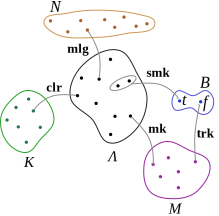
\includegraphics[scale=1.0]{diagramCars}
  \caption{The set $M$ contains all possible makes of cars: Ford,
    Toyota, etc.}
  \label{fig:diagramCars}
\end{figure}

The diagram in the Figure \ref{fig:diagramCars} shows the set $M$ -- the set
of all possible makes of cars. A mapping $\btc{trk}$ returns $true$ if a
given car maker produces trucks.

\subsubsection*{Exercise \ref{exe:relationsGeneral}}
\begin{figure}[htbp]
  \centering
  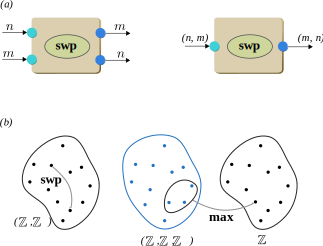
\includegraphics[scale=1.0]{diagramProductSet}
  \caption{(a) Two inputs (outputs) of a function can be replaced with
    a single input of a \bem{pair} of numbers, turning a binary
    function into a unary one. (b) That.}
  \label{fig:diagramProductSet}
\end{figure}

Any binary function can be viewed as a unary function
if two inputs are replaced by a single input of a \emph{pair of
numbers}. Similarly for a function with two outputs. This idea is
illustrated in the Figure \ref{fig:diagramProductSet}(a): The function
{\bf swp} is viewed as a unary function which swaps the numbers in an
\emph{ordered pair}:
\[
\textbf{ swp }\,(n,m) = (m, n)\,.
\]

Given the set $\mathbb{Z}$ of whole numbers, we can create the set of
all possible \emph{ordered pairs} $(n,m)$. This set can be denoted as
follows:
\[
(\mathbb{Z}, \mathbb{Z})\,\textrm{ or }\, \mathbb{Z}\times\mathbb{Z}\,.
\]

The latter notation is standard in mathematics, but the former way
of writing is also acceptable. We can similarly denote the set of all
\emph{ordered triples}:
\[
(\mathbb{Z}, \mathbb{Z}, \mathbb{Z})\,\textrm{ or }\, \mathbb{Z}\times\mathbb{Z}\times\mathbb{Z}\,.
\]

With the notation introduced above, the action of functions with
multiple inputs or outputs can be depicted on the level of sets. The
 Figure \ref{fig:diagramProductSet}(b) shows how this works for the
 functions $\textbf{ swp }$ and $\textbf{ max }$.




%----------------------------------------------------------------------------------------
%	BIBLIOGRAPHY
%----------------------------------------------------------------------------------------

%% \chapter*{Bibliography}
%% \addcontentsline{toc}{chapter}{\textcolor{ocre}{Bibliography}}
%% \section*{Books}
%% \addcontentsline{toc}{section}{Books}
%% \printbibliography[heading=bibempty,type=book]
%% \section*{Articles}
%% \addcontentsline{toc}{section}{Articles}
%% \printbibliography[heading=bibempty,type=article]

%% \cleardoublepage
%% \phantomsection
%% \section*{About Author}

\begin{minipage}{0.3\textwidth}
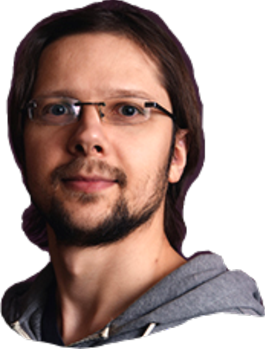
\includegraphics[scale=0.5]{Pictures/yuryd}
\end{minipage}
\begin{minipage}{0.6\textwidth}\raggedright
Yury Deshko is an American applied physicist, educator, and writer.
He is the author of textbook \emph{``Special Relativity For Inquiring Minds''}
aimed at undergraduate students and motivated
high-schoolers.

When not doing applied physics in silicon photonics,
he develops and teaches modern physics courses (Special Relativity and
Quantum Physics) in summer schools for young aspiring physicists.
\end{minipage}
\noindent
\\

%----------------------------------------------------------------------------------------
%	INDEX
%----------------------------------------------------------------------------------------

\cleardoublepage
\phantomsection
\setlength{\columnsep}{0.75cm}
\addcontentsline{toc}{chapter}{\textcolor{ocre}{Index}}
\printindex

%----------------------------------------------------------------------------------------
%% %  back cover
%% \begingroup
%% \thispagestyle{empty}
%% \begin{tikzpicture}[remember picture,overlay]
%% \coordinate [below=0cm] (midpoint) at (current page.north);
%% \node at (current page.north west)
%% {\begin{tikzpicture}[remember picture,overlay]
%% \node[anchor=north west,inner sep=0pt] at (0,0) {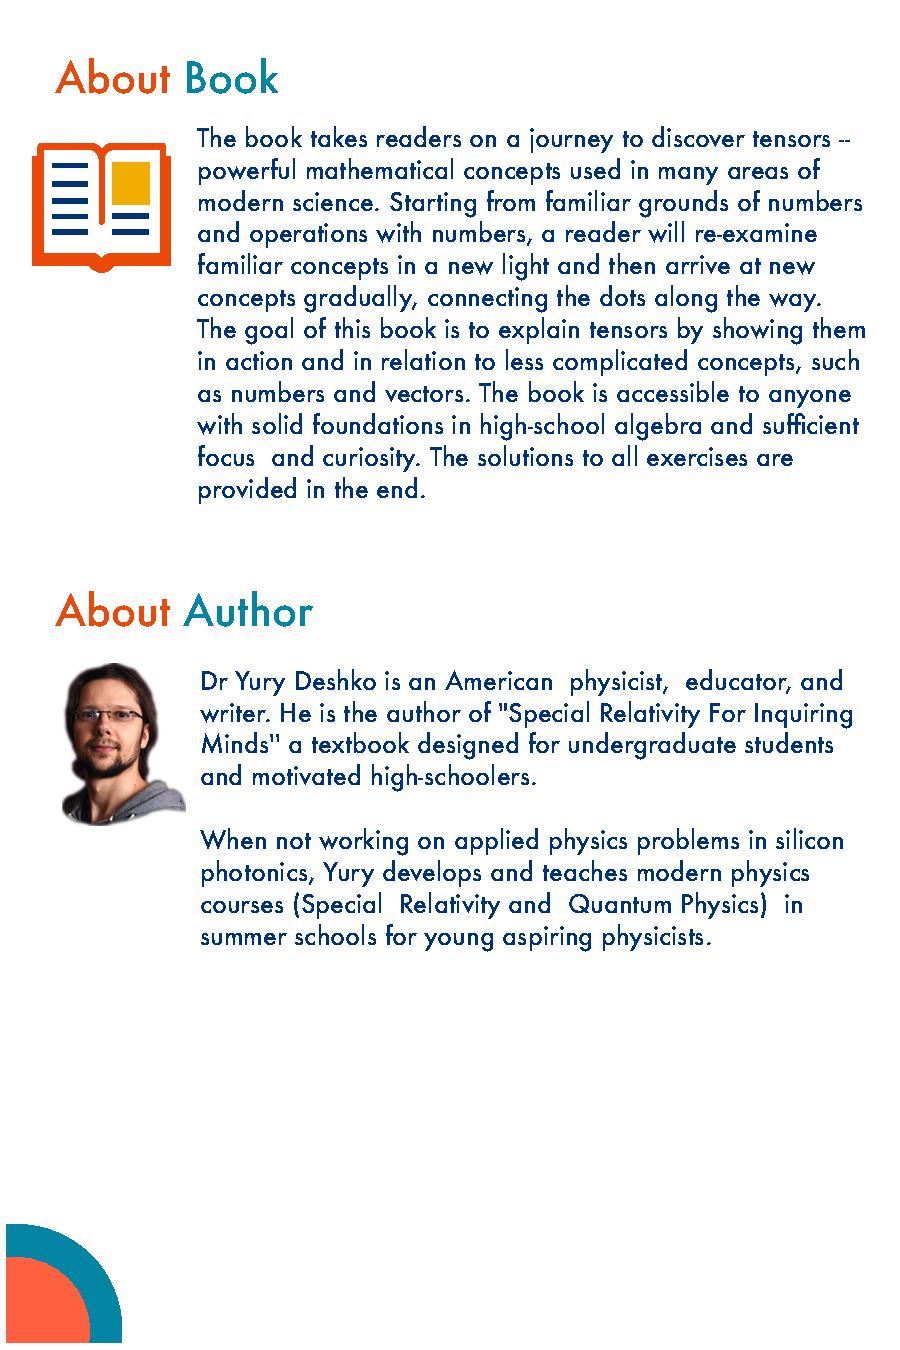
\includegraphics[width=\paperwidth]{Pictures/bookCoverBack_Var1}}; % Background image
%% %\draw[anchor=north] (midpoint) node [fill=ocre!30!white,fill opacity=0.6,text opacity=1,inner sep=1cm]{\Huge\centering\bfseries\sffamily\parbox[c][][t]{\paperwidth}{\centering Relativity\\[15pt] % Book title
%% %{\Large For the Inquiring Mind}\\[20pt] % Subtitle
%% %{\huge Dr. Yury Deshko}}}; % Author name
%% \end{tikzpicture}};
%% \end{tikzpicture}
%% \vfill
%% \endgroup

\end{document}

%%% Local Variables:
%%% mode: latex
%%% TeX-master: t
%%% End:
